%        File: arfc-beamer.tex
%     Created: Sun May 5 10:00 PM 2013 C


%\documentclass[11pt,handout]{beamer}
\documentclass[8pt]{beamer}
\usetheme[white]{Illinois}
%\title[short title]{long title}
\title[Moltres Advancement]{Advancements in Moltres for Time-Dependent Multiphysics Molten Salt
Reactor Modeling}
%\subtitle[short subtitle]{long subtitle}
\subtitle[Final]{Final Examination}
%\subtitle[Brief Summary]{A Brief Summary}
%\author[short name]{long name}
\author[Authors]{Sun Myung Park\\Advanced Reactors and Fuel Cycles Group}
%\date[short date]{long date}
\date[12.12.2024]{December 12, 2024}
%\institution[short name]{long name}
\institute{
  Nuclear, Plasma \& Radiological Engineering\\University of
Illinois Urbana-Champaign}

%\usepackage{bbding}
\usepackage{amsfonts}
\usepackage{amsmath}
\usepackage{amssymb}
\usepackage{mathtools}
\usepackage{bm}
\usepackage{stmaryrd}
\usepackage{xspace}
\usepackage{xcolor}
\usepackage{graphicx}
\graphicspath{{../images/}}
\usepackage{subcaption}
\usepackage{multirow}
\usepackage{siunitx}
\usepackage{booktabs} % nice rules for tables
\usepackage{colortbl}
\usepackage{microtype} % if using PDF
\usepackage{bigints}
\usepackage{minted}
\usepackage[absolute,overlay]{textpos}
\usepackage{tikz}
\usepackage{tkz-euclide}
\usetikzlibrary{positioning, arrows, decorations, shapes, fit, backgrounds}
\usetikzlibrary{shapes.geometric,arrows}
\definecolor{illiniblue}{HTML}{B1C6E2}
\definecolor{illiniorange}{HTML}{f8c2a2}
\definecolor{green}{HTML}{c2e2b1}
\tikzstyle{process} = [rectangle, rounded corners, thick, minimum width=7cm, minimum height=1cm, text centered, draw=black, fill=illiniblue, text width=18em]
\tikzstyle{object} = [ellipse, minimum width=2cm, thick, minimum height=2.2cm, text centered, draw=black, fill=illiniorange, text width=12em]
\tikzstyle{decision} = [diamond, thick, aspect=2, minimum width=2cm, minimum height=2cm, text centered, draw=black, fill=green, text width=6em]
\tikzstyle{arrow} = [thick,->,>=stealth]
\tikzstyle{solver} = [rectangle, rounded corners, thick, minimum width=3cm, minimum height=1.5cm, text centered, draw=black, fill=illiniblue, text width=7em]
\tikzstyle{bound} = [rectangle, rounded corners, thick, draw=black]
\tikzstyle{solver2} = [rectangle, rounded corners, thick, minimum width=2cm, minimum height=1cm, text centered, draw=black, fill=illiniblue, text width=5em]
\tikzstyle{bound} = [rectangle, rounded corners, thick, draw=black]

\usepackage[utf8]{inputenc}
\usepackage[english]{babel}
\usepackage[bibstyle=ieee,backend=bibtex8,sorting=none,eprint=false,isbn=false,doi=false]{biblatex}
\usepackage{textalpha}
\addbibresource{../bibliography.bib}
\AtEveryBibitem{%
  \clearfield{note}%
}
\renewcommand*{\bibfont}{\tiny}

\newcommand{\units}[1] {\:\text{#1}}%
\newcommand{\SN}{S$_N$}%{S$_\text{N}$}%{$S_N$}%
\DeclareMathOperator{\erf}{erf}
%I need some complimentary error functions... 
\DeclareMathOperator{\erfc}{erfc}
%Those icons in the references are terrible looking
\setbeamertemplate{bibliography item}[text]
%Figure numbering
\setbeamertemplate{caption}[numbered]
\setbeamerfont{caption}{size=\small}

%%%% Acronym support

\usepackage[acronym,toc]{glossaries}
\include{acros}


%try to get rid of header on title page\dots
\makeatletter
    \newenvironment{withoutheadline}{
        \setbeamertemplate{headline}[default]
        \def\beamer@entrycode{\vspace*{-\headheight}}
    }{}
\makeatother

\makeatother
\setbeamertemplate{footline}
{
  \leavevmode%
  \hbox{%
    \rightline{\insertframenumber{} / \inserttotalframenumber\hspace*{1ex}}
  }%
  \vskip0pt%
}
\makeatletter
\begin{document}
%%%%%%%%%%%%%%%%%%%%%%%%%%%%%%%%%%%%%%%%%%%%%%%%%%%%%%%%%%%%%
%% From uw-beamer Here's a handy bit of code to place at 
%% the beginning of your presentation (after \begin{document}):
\newcommand*{\alphabet}{ABCDEFGHIJKLMNOPQRSTUVWXYZabcdefghijklmnopqrstuvwxyz}
\newlength{\highlightheight}
\newlength{\highlightdepth}
\newlength{\highlightmargin}
\setlength{\highlightmargin}{2pt}
\settoheight{\highlightheight}{\alphabet}
\settodepth{\highlightdepth}{\alphabet}
\addtolength{\highlightheight}{\highlightmargin}
\addtolength{\highlightdepth}{\highlightmargin}
\addtolength{\highlightheight}{\highlightdepth}
\newcommand*{\Highlight}{\rlap{\textcolor{HighlightBackground}{\rule[-\highlightdepth]{\linewidth}{\highlightheight}}}}
%%%%%%%%%%%%%%%%%%%%%%%%%%%%%%%%%%%%%%%%%%%%%%%%%%%%%%%%%%%%%
%%--------------------------------%%
\begin{withoutheadline}
\frame{
  \titlepage
}
\end{withoutheadline}

%%--------------------------------%%
\AtBeginSection[]{
\begin{frame}
  \frametitle{Outline}
  \tableofcontents[currentsection]
\end{frame}
}

\begin{frame}
  \frametitle{Outline}
  \tableofcontents
\end{frame}

\section{Introduction}
\subsection{Molten Salt Reactors}
%\begin{frame}
%  \frametitle{What is a Molten Salt Reactor (MSR)?}
%	\begin{itemize}
%	  \item Advanced nuclear reactor fueled by fissile
%		material dissolved in a molten salt mixture
%	  \item In most MSR designs, the fuel salt mixture doubles as the primary coolant for the
%        reactor
%	  \item Both thermal- and fast-spectrum configurations are viable
%	\end{itemize}
%	\begin{figure}
%	  \centering
%	  \includegraphics[width=.5\textwidth]{./images/msr}
%      \caption{Schematic diagram of a general channel-type MSR concept
%      \cite{u.s._doe_nuclear_energy_research_advisory_committee_technology_2002}.}
%	  \label{fig:msr}
%	\end{figure}
%\end{frame}

\begin{frame}
  \frametitle{Molten Salt Reactor Modeling \& Simulation}
  \textbf{What is a Molten Salt Reactor (MSR)?}
  \begin{itemize}
	\item MSRs are advanced nuclear reactors fueled by fissile
	  material dissolved in a molten salt mixture.
    \item While modeling MSRs is not necessarily more difficult than modeling solid-fueled
      reactors, we must adapt our software tools to accurately model phenomena unique to MSRs.
  \end{itemize}

  \textbf{Phenomena that pose challenges for MSR modeling}
  \begin{itemize}
	\item Strong multiphysics interactions involving neutron flux, temperature, and flow in the
      reactor core
	  \begin{itemize}
		\item Strong temperature feedback due to thermal expansion of liquid fuel salt
		\item Movement of \glspl{DNP} along primary coolant loop
        \item Advection-dominated heat transfer
	  \end{itemize}
    \item Loss of delayed neutrons to out-of-core decay
    \item Complex turbulent flow effects in MSRs
  \end{itemize}
\end{frame}


\subsection{Moltres}
\input{moltres}
\subsection{Objectives}
\begin{frame}
  \frametitle{Objectives}
  \begin{block}{\textbf{Overarching Goal of this Work}}
    Improve Moltres as a MSR simulation tool by enabling a wider range of MSR simulation
    scenarios.
  \end{block}
  \begin{block}{\textbf{Objectives}}
    \begin{enumerate}
      \item \textbf{Improve Multiphysics Capabilities in Moltres}
      \begin{itemize}
        \item Verify and validate existing multiphysics coupling capabilities in Moltres
        \item Implement a RANS-based turbulence model in Moltres
      \end{itemize}
      \item \textbf{Develop a Hybrid Neutronics Method for Control Rod Modeling in Moltres}
      \begin{itemize}
        \item Develop and implement the hybrid $S_N$-diffusion method in Moltres
        \item Verify the hybrid method against high-fidelity neutronics codes and MSRE
          experimental data
        \item Demonstrate a time-dependent reactivity-initiated simulation using the hybrid
          method
      \end{itemize}
    \end{enumerate}
  \end{block}
\end{frame}


\section{Objective 1: Improve Multiphysics Coupling Capabilities}
\subsection{V\&V Study: MSRE Pump Start-up \& Coast-Down Transients}
\begin{frame}
  \frametitle{Description of MSRE Pump Experiments}
  \begin{itemize}
    \item Starting from zero-power critical states under static/steady-flow conditions, the fuel salt pump
  was started up/coasted down.
    \item Reactor was kept critical by a flux-servo controller moving the rod in response to flux
      changes.
  \end{itemize}
  \begin{block}{\textbf{MSR Physics Phenomena Involved}}
    \begin{itemize}
      \item DNP drift under time-varying flow
      \item Loss of delayed neutrons due to out-of-core DNP decay
    \end{itemize}
  \end{block}
  \begin{columns}
    \column{5.5cm}
    \begin{figure}
      \centering
      \includegraphics[width=.8\columnwidth]{images/msre-startup}
      \caption{MSRE start-up pump speed and flow rate
      \cite{prince_zero-power_1968}.}
    \end{figure}
    \column{5.5cm}
    \begin{figure}
      \centering
      \includegraphics[width=.95\columnwidth]{images/msre-coastdown}
      \caption{MSRE coast-down pump speed and flow rate
      \cite{prince_zero-power_1968}.}
    \end{figure}
  \end{columns}
\end{frame}

%\begin{frame}
%  \frametitle{V\&V Study 2: MSRE Pump Start-up \& Coast-Down Transients}
%  \begin{block}{\textbf{MSR Phenomena Involved}}
%    \begin{itemize}
%      \item DNP drift under time-varying flow
%      \item Loss of delayed neutrons due to out-of-core DNP decay
%    \end{itemize}
%  \end{block}
%  \begin{block}{\textbf{Aim of the Study}}
%    Reproduce the reactivity curve of the control rod response with a 2-D axisymmetric model of the
%    MSRE in Moltres.
%  \end{block}
%  \begin{block}{\textbf{Study Objectives}}
%    \begin{itemize}
%      \item Develop a V\&V study based on the MSRE pump start-up \& coast-down
%        transients that is easily reproducible
%      \item Verify Moltres against QuasiMolto in collaboration with Aaron Reynolds
%        (formerly at Oregon State University)
%      \item Validate Moltres against MSRE experimental data for modeling \gls{DNP} drift
%    \end{itemize}
%  \end{block}
%\end{frame}

\begin{frame}
  \frametitle{V\&V Study: MSRE Pump Start-up \& Coast-Down Transients}
  \begin{columns}
    \column{6.5cm}
    \begin{block}{\textbf{Aim of the Study}}
      \begin{itemize}
         \item Develop a verification and validation (V\&V) study based on the MSRE pump transients
         \item Verify Moltres against QuasiMolto \cite{reynolds_analysis_2023} in collaboration
           with Dr.\ Aaron Reynolds
         \item Validate Moltres against MSRE experimental data for modeling \gls{DNP} drift
       \end{itemize}
    \end{block}
    \begin{block}{\textbf{Modeling Approach}}
      \begin{itemize}
        \item Two neutron energy groups and six DNP groups
        \item Ignored upper and lower plena in the geometry
%        \item Looped salt flow with a salt circulation time of 25.2 s
        \item $k$-eigenvalue calculation at every time-step ($dt=0.1$ s) in place of reactivity control
      \end{itemize}
    \end{block}
    \column{4.5cm}
    \begin{figure}[htb]
      \centering
      \includegraphics[width=0.8\columnwidth]{images/msre-2d-pres}
      \caption{2-D axisymmetric model of the \gls{MSRE}.The gray and white regions represent fuel salt
      and graphite, respectively. Fuel salt channels are 1.25-cm wide and spaced at 5-cm intervals.}
      \label{fig:pump-geom}
    \end{figure}
  \end{columns}
\end{frame}

\begin{frame}
  \frametitle{MSRE $k_\text{eff}$ Estimates Under Static \& Steady-Flow Conditions}
  \begin{table}[htb]
    \centering
    \caption{Multiplication factors $k_\text{eff}$ under static and steady salt flow conditions, and
    reactivity changes $\Delta\rho$ due to \gls{DNP} flow from the Moltres and QuasiMolto \gls{MSRE}
    models.}
    \begin{tabular}{l S S S}
      \toprule
      \multirow{2}{*}{Code} & \multicolumn{2}{c}{$k_\text{eff}$} & {$\Delta\rho$ due to} \\
                            & {Static} & {Steady flow} & {\gls{DNP} flow} \\
                            \cmidrule(r){1-1} \cmidrule(rl){2-3} \cmidrule(l){4-4}
      Moltres & 1.05625 & 1.05311 & -282.4 \\
      QuasiMolto & 1.05603 & 1.05290 & -281.7 \\
      \bottomrule
    \end{tabular}
    \label{table:msre-pump-keff}
  \end{table}
  \begin{itemize}
    \item Excellent agreement between Moltres and QuasiMolto under static and steady-flow conditions prior
  to the pump transients.
  \end{itemize}
\end{frame}

\begin{frame}
  \frametitle{MSRE Neutron Flux Distributions Under Static Conditions}
  \begin{figure}[h]
    \centering
    \begin{subfigure}[b]{0.48\columnwidth}
      \centering
      \includegraphics[width=\columnwidth]{centerline_flux}
      \caption{Normalized centerline neutron fluxes.}
      \label{fig:centerline-flux-dist}
    \end{subfigure}
    \hfill
    \begin{subfigure}[b]{0.48\columnwidth}
      \centering
      \includegraphics[width=\columnwidth]{midplane_flux}
      \caption{Normalized midplane neutron fluxes.}
      \label{fig:midplane-flux-dist}
    \end{subfigure}
    \caption{Neutron flux distributions comparing QuasiMolto and Moltres
    \gls{MSRE} models under static conditions. Maximum relative difference $\approx 0.8 \%$.}
    \label{fig:centerline-flux}
  \end{figure}
  \begin{itemize}
    \item Perfect overlap in centerline and midplane neutron fluxes between Moltres and QuasiMolto.
  \end{itemize}
\end{frame}

\begin{frame}
  \frametitle{MSRE Pump Start-Up Transient Results}
  \begin{columns}
  \column{5.5cm}
  \begin{figure}[t]
    \centering
    \includegraphics[width=\columnwidth]{start-up-v2-reactivity}
    \caption{Reactivity loss (relative to static conditions) during the \gls{MSRE} pump
    start-up transient.}
    \label{fig:start-up-reactivity}
  \end{figure}
  \column{5.5cm}
  \textbf{Numerical Results}
  \begin{itemize}
    \item Reactivity loss plateaus after excess DNPs exit.
    \item Circulation of the excess DNPs cause reactivity oscillations that eventually dissipate.
    \item Excellent agreement between Moltres and QuasiMolto.
  \end{itemize}
  \pause
  \textbf{Discrepancies against MSRE Data}
  \begin{itemize}
    \item MSRE had a smaller final reactivity loss.
    \item MSRE did not report a reactivity plateau (due to DNPs present in the upper and lower plena).
    \item MSRE did not log significant reactivity oscillations after the first peak.
  \end{itemize}
  \end{columns}
\end{frame}

%\begin{frame}
%  \frametitle{V\&V Study 2: MSRE Pump Start-up \& Coast-Down Transients}
%  \textbf{Pump Start-Up Transient Results}
%  \begin{columns}
%  \column{5.5cm}
%  \begin{figure}[t]
%    \centering
%    \includegraphics[width=\columnwidth]{start-up-v2-reactivity}
%    \caption{Reactivity loss (relative to static no-flow conditions) during the \gls{MSRE} pump
%    start-up transient.}
%    \label{fig:start-up-reactivity}
%  \end{figure}
%  \column{5.5cm}
%  \textbf{Discrepancies against MSRE Data}
%  \begin{itemize}
%    \item MSRE reported a smaller final reactivity loss
%    \item MSRE did not report a reactivity plateau (due to DNP present in the upper and lower plena)
%    \item MSRE did not log significant reactivity oscillations after the first peak
%  \end{itemize}
%  \end{columns}
%\end{frame}

\begin{frame}
  \frametitle{Pump Coast-Down Transient Results}
  \begin{figure}[t]
    \centering
    \includegraphics[width=.7\columnwidth]{coast-down-v2-reactivity}
    \caption{Reactivity loss (relative to static no-flow conditions) during the \gls{MSRE} pump
    coast-down transient.}
    \label{fig:start-up-reactivity}
  \end{figure}
  Good agreement between numerical and experimental data other than the magnitude differences.
\end{frame}

\begin{frame}
  \frametitle{Summary: MSRE Pump Start-up \& Coast-Down Transients}
  \begin{block}{\textbf{Study Outcome}}
    \begin{itemize}
      \item Moltres and QuasiMolto are highly consistent with each other in their looped DNP flow
        modeling capabilities
      \item Moltres and QuasiMolto reproduced key reactivity behavior in response to varying salt
        flow velocities
      \item Some discrepancies observed between the numerical and experimental results due to the
        omission of upper and lower plena
      \item This study can be used for verifying advection capabilities in other MSR simulation tools
      \item The distinct oscillations serve as valuable reference points to facilitate code-to-code
        comparisons
    \end{itemize}
  \end{block}
\end{frame}

\subsection{Motivation for Turbulence Modeling Implementation}
\input{turb-motivation}
\subsection{Spalart-Allmaras Turbulence Model in Moltres}
\begin{frame}
  \frametitle{Spalart-Allmaras Turbulence Model in Moltres}
  \begin{block}{\textbf{Why the Spalart-Allmaras Model for Moltres?}}
    A computationally efficient one-equation model that provides reasonable estimates for turbulent
    effects in MSRs and is tractable for large problems on small computing clusters.
  \end{block}
  \begin{block}{\textbf{Subobjectives}}
    \textbf{Implementation of a Spalart-Allmaras turbulence model in Moltres}
    \begin{itemize}
      \item Implement a Spalart-Allmaras model in Moltres
      \item Verify and validate the model against reference turbulent flow solutions
    \end{itemize}
  \end{block}
\end{frame}

\begin{frame}
  \frametitle{Spalart-Allmaras Turbulence Model in Moltres}
  \textbf{Spalart-Allmaras Model with Rotation Correction Scheme
  \cite{spalart_one-equation_1994, aupoix_extensions_2003, dacles-mariani_numericalexperimental_1995}}\\
  \\
  Governing equation for the modified dynamic viscosity, $\tilde{\mu}$:
  \begin{multline}
    \rho \frac{\partial\tilde{\mu}}{\partial t} + \rho \mathbf{u}\cdot\nabla\tilde{\mu} = \rho c_{b1}
    \left(1-f_{t2}\right)\tilde{S}\tilde{\mu} + \frac{1}{\sigma}\{\nabla\cdot\left[\left(\mu+
    \tilde{\mu}\right)\nabla\tilde{\mu}\right] + c_{b2}|\nabla\tilde{\mu}|^2\} \\
    - \left(c_{w1}f_w - \frac{c_{b1}}{\kappa^2}f_{t2}\right)\left(\frac{\tilde{\mu}}{d}\right)^2
  \end{multline}
  \begin{align*}
    \shortintertext{where}
      \mu_t &= \tilde{\mu}f_{v1} = \text{turbulent eddy viscosity}, \\
      f_{v1} &= \frac{\chi^3}{\chi^3 + c_{v1}^3}, \\
      \chi &= \frac{\tilde{\mu}}{\mu}.
  \end{align*}
%      \tilde{S} &= \Omega + \frac{\tilde{\nu}}{\kappa^2 d^2} f_{v2}, \\
%      f_{v2} &= 1 - \frac{\chi}{1+\chi f_{v1}}, \\
%      \Omega &= \sqrt{2W_{ij}W_{ij}} = \text{vorticity magnitude}, \\
%      W_{ij} &= \frac{1}{2}\left(\frac{\partial u_i}{\partial x_j} - \frac{\partial u_j}{\partial x_i}
%      \right), \\
%        f_w &= g\left(\frac{1 + c_{w3}^6}{g^6 + c_{w3}^6}\right)^{1/6}, \\
%        g &= r + c_{w2}\left(r^6 - r\right), \\
%        r &= \text{min}\left(\frac{\tilde{\nu}}{\tilde{S}\kappa^2d^2}, 10\right), \\
%        f_{t2} &= c_{t3} \exp{\left(-c_{t4}\chi^2\right)},
%    \end{align*}
%  \shortintertext{and the constants are}
%    \sigma = \frac{2}{3}, \ c_{b1} = 0.1355, \ c_{b2} = 0.622, \ \kappa = 0.41, \
%    c_{w1} = \frac{c_{b1}}{\kappa^2} + \frac{1+c_{b2}}{\sigma}, \nonumber \\
%    c_{w2} = 0.3, \ c_{w3} = 2, \
%    c_{v1} = 7.1, \ c_{t3} = 1.2, \ c_{t4} = 0.5 \ \text{.} \nonumber
\end{frame}

\begin{frame}
  \frametitle{Spalart-Allmaras Turbulence Model in Moltres}
  \begin{block}{\textbf{Model Implementation Details}}
  \begin{itemize}
    \item Built on top of an existing incompressible Navier-Stokes model in MOOSE
    \item Uses \gls{SUPG} stabilization scheme for numerical stability
    \item $f_{t2}$ turbulence trip term is togglable (Negligible difference in fully turbulent flows)
    \item Rotation correction scheme \cite{aupoix_extensions_2003, dacles-mariani_numericalexperimental_1995}
      reduces eddy viscosity in regions of rotational but non-turbulent flow
  \end{itemize}
  \end{block}
  \pause
  \begin{block}{\textbf{Verification \& Validation Tests for the Turbulence Model}}
    \begin{enumerate}
      \item Turbulent Channel Flow Verification Test at Re $\approx 13750$
      \begin{itemize}
        \item Reference results: \gls{DNS} results by Moser et al.\ \cite{moser_direct_1999}
      \end{itemize}
      \item Turbulent Pipe Flow Validation Test at Re $\approx 40000$
      \begin{itemize}
        \item Reference results: Experimental results by Laufer \cite{laufer_structure_1954}
      \end{itemize}
      \item Backward-Facing Step Flow Validation Test
      \begin{itemize}
        \item Reference results: Experimental results by Driver \& Seegmiller \cite{driver_features_1985}
        \item Reference results: Spalart-Allmaras model results from CFL3D CFD code \cite{krist_cfl3d_1998}
      \end{itemize}
    \end{enumerate}
  \end{block}
\end{frame}

\begin{frame}
  \frametitle{Spalart-Allmaras Turbulence Model in Moltres}
  \textbf{Turbulent Channel Flow Verification Test Results}
  \begin{figure}[htb!]
    \centering
    \begin{subfigure}[b]{0.32\columnwidth}
      \centering
      \includegraphics[width=\columnwidth]{channel_vel}
      \caption{Normalized velocity distribution across the channel.}
      \label{fig:channel-vel}
    \end{subfigure}
    \hfill
    \begin{subfigure}[b]{0.32\columnwidth}
      \centering
      \includegraphics[width=\columnwidth]{channel_nondim}
      \caption{Dimensionless velocity vs.\ dimensionless wall distance.}
      \label{fig:channel-nondim}
    \end{subfigure}
    \begin{subfigure}[b]{0.32\columnwidth}
      \centering
      \includegraphics[width=\columnwidth]{channel_stress}
      \caption{Normalized stress distribution across the channel.}
      \label{fig:channel-stress}
    \end{subfigure}
    \caption{Comparison of turbulent channel flow results at Re$_\tau\approx395$ against reference
    \gls{DNS} results \cite{moser_direct_1999}. The Moltres Spalart-Allmaras model agrees consistently with
    the reference data.}
    \label{fig:channel-verification}
  \end{figure}
\end{frame}

\begin{frame}
  \frametitle{Spalart-Allmaras Turbulence Model in Moltres}
  \textbf{Turbulent Pipe Flow Validation Test Results}
  \begin{figure}[htb]
    \centering
    \begin{subfigure}[b]{0.32\columnwidth}
      \centering
      \includegraphics[width=\columnwidth]{pipe_vel}
      \caption{Normalized velocity distribution across the pipe.}
      \label{fig:pipe-vel}
    \end{subfigure}
    \hfill
    \begin{subfigure}[b]{0.32\columnwidth}
      \centering
      \includegraphics[width=\columnwidth]{pipe_nondim}
      \caption{Dimensionless velocity vs.\ dimensionless wall distance}
      \label{fig:pipe-nondim}
    \end{subfigure}
    \begin{subfigure}[b]{0.32\columnwidth}
      \centering
      \includegraphics[width=\columnwidth]{pipe_stress}
      \caption{Normalized turbulent shear stress across the pipe.}
      \label{fig:pipe-stress}
    \end{subfigure}
    \caption{Comparison of turbulent pipe flow results at Re $\approx 40000$ against reference
    experimental data \cite{laufer_structure_1954}.}
    \label{fig:pipe-verification}
  \end{figure}
\end{frame}

\begin{frame}
  \frametitle{Spalart-Allmaras Turbulence Model in Moltres}
  \textbf{Backward-Facing Step Flow Validation Test Results}
  \begin{columns}
    \column{5.5cm}
    \begin{figure}[h]
      \centering
      \includegraphics[width=\columnwidth]{backstep-geom-pres}
      \caption{Backward step geometry for the turbulent BFS flow verification test. The red box indicates
      the region shown by the close-up view in Figure \ref{fig:bfs-mesh}.}
      \label{fig:backstep-geom}
    \end{figure}
    \column{5.5cm}
    \begin{figure}[h]
      \centering
      \includegraphics[width=\columnwidth]{bfs_mesh}
      \caption{Close-up view of the mesh for the BFS flow test. The step is situated at $x=110$ m
      with a height of $H=1$ m.}
      \label{fig:bfs-mesh}
    \end{figure}
  \end{columns}
\end{frame}

\begin{frame}
  \frametitle{Spalart-Allmaras Turbulence Model in Moltres}
  \textbf{Backward-Facing Step Flow Validation Test Results}
  \begin{columns}
    \column{5.5cm}
    \begin{figure}[htb!]
      \centering
      \includegraphics[width=\columnwidth]{bfs}
      \caption{Velocity magnitude distribution and streamlines around the backward-facing step. The
      streamlines illustrate the primary and secondary recirculation zones.}
      \label{fig:bfs}
    \end{figure}
    \column{5.5cm}
    \begin{table}[htb]
      \centering
      \scriptsize
      \caption{BFS flow reattachment length estimates normalized by step height $H$.}
      \begin{tabular}{l S[table-format=1.2(2)]}
        \toprule
        Source & {Reattachment length [-]} \\
        \midrule
        Experimental data & 6.26(10) \\
        CFL3D & 6.1 \\
        Moltres & 6.36 \\
        \bottomrule
      \end{tabular}
      \label{table:bfs-reattach}
    \end{table}
  \end{columns}
\end{frame}

\begin{frame}
  \frametitle{Spalart-Allmaras Turbulence Model in Moltres}
  \textbf{Backward-Facing Step Flow Validation Test Results}
  \begin{figure}[htb]
    \centering
    \hfill
    \begin{subfigure}[b]{0.24\columnwidth}
      \centering
      \includegraphics[width=\columnwidth]{bfs_downstream_vel}
      \caption{Normalized velocity distributions downstream of step.}
      \label{fig:bfs-downstream}
    \end{subfigure} %\hfill \\
%    \centering
    \hfill
    \begin{subfigure}[b]{0.24\columnwidth}
      \centering
      \includegraphics[width=\columnwidth]{bfs_cf}
      \caption{Skin friction coefficient along the bottom wall.}
      \label{fig:bfs-cf}
    \end{subfigure}
    \hfill
    \begin{subfigure}[b]{0.24\columnwidth}
      \centering
      \includegraphics[width=\columnwidth]{bfs_cp}
      \caption{Skin pressure coefficient along the bottom wall.}
      \label{fig:bfs-cp}
    \end{subfigure}% \hfill \\
%    \centering
    \begin{subfigure}[b]{0.24\columnwidth}
      \centering
      \includegraphics[width=\columnwidth]{bfs_stress}
      \caption{Normalized turbulent shear stress downstream
      of step.}
      \label{fig:bfs-stress}
    \end{subfigure}
    \caption{Comparison of backward facing step flow results against reference
    experimental data and computational data from CFL3D. $x/H$ values are normalized horizontal
    distances relative to the step.}
    \label{fig:bfs-plots}
  \end{figure}
\end{frame}

\begin{frame}
  \frametitle{Spalart-Allmaras Turbulence Model in Moltres}
  \textbf{Spalart-Allmaras Model V\&V Test Summary}
  \begin{itemize}
    \item Good agreement between Moltres and reference solutions in the turbulent channel and pipe
      flow tests
    \item Good agreement between Moltres and CFL3D in the backward-facing step flow test
    \item Some discrepancy between Moltres and experimental data in the backward-facing step flow
      test, but Moltres performed better than CFL3D at predicting flow reattachment length and
      velocity/stress distributions along $x/H=1$.
  \end{itemize}
\end{frame}


\section{Objective 2: Hybrid $S_N$-Diffusion Method}
\subsection{Motivation}
\begin{frame}
  \frametitle{Control Rods in MSRs}
  \begin{columns}
    \hfill
    \column[t]{5cm}
    \vspace{.2cm}
    \begin{figure}
      \centering
      \includegraphics[width=\columnwidth]{images/msre-cutout}
      \caption{\footnotesize MSRE reactor vessel \cite{robertson_msre_1965}}
    \end{figure}
    \hfill
    \column[t]{6cm}
    \begin{figure}
      \centering
      \includegraphics[width=.8\columnwidth]{images/tmsr}
      \caption{\footnotesize Cross-sectional views of the TMSR-LF1
      \cite{liu_sensitivityuncertainty_2020}}
    \end{figure}
    \begin{figure}
      \centering
      \includegraphics[width=.5\columnwidth]{images/tap-msr-rods}
      \caption{\footnotesize Cross-sectional view of the TAP MSR \cite{lee_neutronics_2020}}
    \end{figure}
    \hfill
  \end{columns}
\end{frame}

\begin{frame}
  \frametitle{Control Rods in MSRs}
  \textbf{Control rods provide a means of controlling the fission rate in nuclear reactors.} 
  \begin{itemize}
    \item Facilitate reactor start-up, shut-down, or load-following operations
    \item Consist of highly neutron-absorbing materials such as boron or gadolinium
  \end{itemize}
  \textbf{Control rods are also important for licensing and safety characterization.}

  $\Rightarrow$ \textbf{It is important to characterize control rod effects in all relevant
  transient scenarios.}
%  \textbf{Many MSR designs contain comparatively fewer control rods than most other reactor types due to:}
%  \begin{itemize}
%    \item Uniform liquid fuel burnup
%    \item Strong passive safety of the liquid fuel form
%    \item Low excess reactivity of fuel inventory
%    \item Availability of other control mechanisms
%  \end{itemize}

\end{frame}

\begin{frame}
  \frametitle{Control Rod Modeling}
  \textbf{Control rods induce highly anisotropic neutron fluxes and steep flux gradients in their
  vicinity.}
  \begin{block}{\textbf{The Control Rod Modeling Dilemma}}
    \begin{itemize}
      \item Neutron diffusion, $P_1$, and $SP_N$ methods perform poorly near control rod regions
        due to the highly anisotropic neutron fluxes and steep flux gradients
      \item High-fidelity neutron transport methods remain too computationally expensive for
        routine time-dependent multiphysics simulations
    \end{itemize}
  \end{block}
\end{frame}

\begin{frame}
  \frametitle{Control Rod Modeling in MSR Multiphysics Studies}
  \vspace{.2cm}

  Common approximations applied to control rod modeling include:
  \begin{itemize}
    \item Homogenized, coarse-mesh geometries containing static control rods with albedo neutron
      flux boundary conditions \cite{kophazi_development_2009} or transport-corrected cross
      sections \cite{cui_development_2021, jaradat_development_2021, yang_development_2022}
      \begin{itemize}
        \item Neutronics geometry differs from thermal-hydraulics geometry
        \item Static calibration factors may not be suitable for time-dependent simulations
      \end{itemize}
    \item Scaling the neutron source term to simulate moving control rods
      \cite{delpech_benchmark_2003, krepel_dyn3d-msr_2007, jaradat_development_2021,
      yang_development_2022}
      \begin{itemize}
        \item Does not capture local or asymmetric flux changes
      \end{itemize}
  \end{itemize}

  \begin{block}{\textbf{Technical Gap}}
    \textbf{There are no MSR simulation tools or studies that explicitly model moving control rods.}
  \end{block}
\end{frame}

\subsection{Literature Review}
\begin{frame}
  \frametitle{Transport-Correction Techniques For Neutron Diffusion-Based Solvers}
  Techniques for augmenting the neutron diffusion method (or equivalent low-order equations) with
  corrections derived from neutron transport:
  \begin{itemize}
    \item Ronen method \cite{ronen_accurate_2004, tomatis_ronen_2021, gross_comprehensive_2023}
    \item Multilevel quasi-diffusion method \cite{goldin_quasi-diffusion_1964, tamang_multilevel_2014, reynolds_analysis_2023}
    \item Multischeme transport method \cite{wang_hybrid_2017}
    \item Hybrid transport-diffusion method \cite{anistratov_computational_2012, stehle_hybrid_2014}
  \end{itemize}
  These techniques generally require:
  \begin{itemize}
    \item High-order neutron transport solver
    \item Corrective terms for the neutron diffusion equations
    \item Boundary coupling scheme (for spatial domain decomposition)
  \end{itemize}
\end{frame}

\begin{frame}
  \frametitle{The Ronen Method}
  \vspace{.2cm}

  Starting with an initial neutron diffusion flux solution, a transport
  expression is used to iteratively improve the flux solution by updating the
  diffusion coefficients:
  %
  \begin{align}
    D(\vec{r},E) =& -\frac{J_{tr}(\vec{r},E)}{\nabla \phi(\vec{r},E)}
    \label{eq:ronen}
    \shortintertext{where}
    J_{tr} =& \mbox{ transport-derived neutron current.} \nonumber
  \end{align}
  %
  In 1-D slab geometry, the integral expression for calculating the current is:
  %
  \begin{align}
    J(x,E) = \frac{1}{2}\int^a_0 dx'\ &E_2[\tau(x',x,E)sgn(x-x')q_0(x',E) \nonumber \\
    &+\frac{3}{2}\int^a_0dx' \ E_3[\tau(x',x,E)]q_1(x',E)
  \end{align}
  \textbf{Limitation: Demonstrated for 1-D geometries only.}
\end{frame}

%\begin{frame}
%  \frametitle{Hybrid $S_N$-Diffusion Method: Literature Review}
%  \textbf{Transport-Derived Diffusion Closures \cite{pounders_diffusion_2009}}
%  \vspace{.2cm}
%  
%  Pounders \& Rahnema developed two separate methods which also
%  generate space-dependent diffusion coefficients for transport corrections.
%  \vspace{.1cm}
%  \begin{columns}
%    \column[t]{.5\textwidth}
%    \textbf{1) Averaged Eddington Factor Diffusion Theory}
%    %
%    \begin{align}
%      \small
%      E_g(z) =& \frac{\int^1_{-1} \mu^2\psi(z,\mu)d\mu}{\int^1_{-1} \psi(z,\mu)d\mu}
%    \end{align}
%    %
%    \begin{align}
%      \small
%      D^{AEF}_g(z) =& E^i_g\left[\hat{\Sigma}_{t,g}-\sum^G_{g'=1}\hat{\Sigma}^{g'\rightarrow g}_{s1}
%      \frac{\hat{J}_{g'}}{\hat{J}_g}\right]^{-1}
%    \end{align}
%    \hfill
%    \column[t]{.5\textwidth}
%    \textbf{2) High-Order Empirical Diffusion Coefficients}
%    \begin{align}
%      D^i_g =& -\frac{\left(z_{i+1}-z_i\right) \bar{J}_g}{\left[\phi_g(z_{i+1})-\phi_g(z_i)\right]}
%      \label{eq:emp}
%    \end{align}
%  \end{columns}
%  \textbf{Limitation: Both methods require a priori knowledge of the neutron flux and current
%  solution.}
%\end{frame}

\begin{frame}
  \frametitle{Multilevel Quasi-Diffusion Method}
  Gol'din originally developed the quasi-diffusion (QD) method as a transport method acceleration
  scheme \cite{goldin_quasi-diffusion_1964}.
  \begin{gather}
    \mbox{\small Zeroth angular moment: } 
    \nabla\cdot J(\vec{r}) + \Sigma_t(\vec{r})\phi(\vec{r}) = \Sigma_{s,0}(\vec{r})\phi(\vec{r}) +
    Q_0(\vec{r}) \label{eq:qd-low-0th} \\
    \mbox{\small First angular moment: }
    \nabla\cdot\left(\vec{\vec{E}}(\vec{r})\phi(\vec{r})\right) + \Sigma_t(\vec{r})J(\vec{r}) =
    \Sigma_{s,1}(\vec{r})J(\vec{r}) + Q_1(\vec{r}) \label{eq:qd-low-1st}
    \shortintertext{\small where}
    \vec{\vec{E}} = \frac{\int_{4\pi}d\hat{\Omega}\ \hat{\Omega}\hat{\Omega}\psi(\vec{r})}{
    \int_{4\pi}d\hat{\Omega}\ \psi(\vec{r})} = \mbox{\small Eddington tensor}.
  \end{gather}
  %
  Gol'din later extended it to a three-level method by deriving effective gray (one-group)
  low-order QD equations \cite{anistratov_solution_1986}.
  \begin{figure}[t]
    \tikzstyle{every node}=[font=\small]
    \centering
    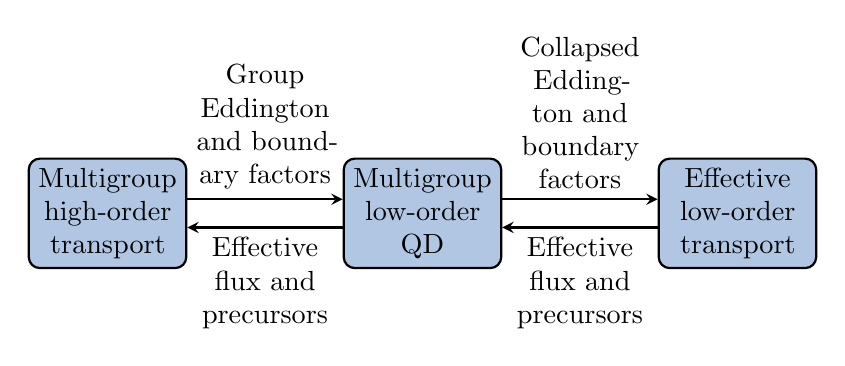
\begin{tikzpicture}
      \node (1) [solver2] {Multigroup high-order transport};
      \node (2) [solver2, right of=1, xshift=3cm] {Multigroup low-order QD};
      \node (3) [solver2, right of=2, xshift=3cm] {Effective low-order transport};
      \draw [arrow] (1.10) -- node[anchor=south, text width=2cm, align=center] {Group\\ Eddington
        and boundary factors} (2.170);
      \draw [arrow] (2.190) -- node[anchor=north, text width=2cm, align=center] {Effective flux
        and precursors} (1.350);
      \draw [arrow] (2.10) -- node[anchor=south, text width=2cm, align=center] {Collapsed Eddington
        and boundary factors} (3.170);
      \draw [arrow] (3.190) -- node[anchor=north, text width=2cm, align=center] {Effective flux
        and precursors} (2.350);
    \end{tikzpicture}
    \caption{Algorithm flowchart for the three-level quasi-diffusion method.}
    \label{fig:algorithm}
  \end{figure}
\end{frame}

\begin{frame}
  \frametitle{Multilevel Quasi-Diffusion Method}
  Tamang \& Anistratov applied the QD method to 1-D time-dependent multiphysics neutron transport
  and heat transfer problems by iteratively coupling the one-group low-order equations to the heat
  transfer and precursor equations \cite{tamang_multilevel_2014}.
  \vspace{.2cm}

  Reynolds \& Palmer applied the same approach for steady-state simulations of a 2-D axisymmetric,
  two-group MSRE model \cite{reynolds_analysis_2023}.
  %
  \begin{figure}[h]
    \centering
    \includegraphics[width=.6\columnwidth]{images/reynolds-flux}
    \caption{Fast and thermal fluxes of the 2-D axisymmetric MSRE model by Reynolds \& Palmer
    \cite{reynolds_analysis_2023}.}
    \label{fig:reynolds-flux}
  \end{figure}
  \textbf{Limitation: Computational expensive for 3-D full-core simulations.}
\end{frame}

\begin{frame}
  \frametitle{Multischeme Transport Method}
  Implemented in the Griffin reactor physics application \cite{wang_hybrid_2017}. This method
  involves making predetermined
  domain decompositions to be treated with the $S_N$, $P_N$, or diffusion methods. Adjoining
  subdomains are coupled through the Lagrange multiplier interface condition:
  \begin{gather}
    -\int_S \left[\left(\llbracket\Psi\rrbracket,\Lambda^*\right)_{\Gamma} +
    \left(\llbracket\Psi^*\rrbracket,\Lambda\right)_{\Gamma}\right] d\hat{\Omega}
    \shortintertext{where}
    \begin{align}
      \llbracket\Psi\rrbracket &= \Psi^+ - \Psi^-, 
      \Psi^\pm = \lim_{s\rightarrow 0^+} \Psi(\vec{x}+s\hat{n}), \nonumber \\
      \Lambda &= \mbox{ Lagrange multiplier},
      \Gamma = \mbox{ interface boundary}, \nonumber \\
      \hat{n} &= \mbox{ normal vector at interface boundary}, \nonumber
    \end{align}
  \end{gather}
  or the upwinding method:
  \begin{gather}
    \int_S \left(|\hat{\Omega}\cdot\hat{n}|\llbracket\Psi^*\rrbracket,\Psi^-\right)_{\Gamma^+}
    d\hat{\Omega} -
    \int_S\left(|\hat{\Omega}\cdot\hat{n}|\llbracket\Psi^*\rrbracket,\Psi^+\right)_{\Gamma^-}
    d\hat{\Omega}
  \end{gather}
\end{frame}

\begin{frame}
  \frametitle{Hybrid Transport-Diffusion Method \cite{anistratov_computational_2012, stehle_hybrid_2014}}
  \vspace{.2cm}

  Anistratov \& Stehle developed an adaptive domain decomposition scheme using Eddington tensor
  estimates as a metric for deducing whether a region is diffusive or
  transport-like.
  \vspace{.2cm}

  It uses two-level neutronics method based on the Second-Moment method \cite{lewis_comparison_1976}.
  The low-order second-moment equations on the $(s+1)$th iteration are:
  \begin{gather}
    \nabla\cdot J^{(s+1)}+\Sigma_a\phi^{(s+1)} = q, \label{eq:2nd-moment-1} \\
    \frac{1}{3}\nabla\cdot\phi^{(s+1)}+\Sigma_t J^{(s+1)} = \nabla\cdot F^{(s+1/2)}
    \label{eq:2nd-moment-2}
    \shortintertext{where}
    F^{(s+1/2)}_{\alpha\beta} = \int_{4\pi}
    \left(\frac{1}{3}\delta_{\alpha\beta}-\Omega_\alpha\Omega_\beta\right)
    \Psi^{(s+1/2)} d\Omega \label{eq:2nd-moment-3}
  \end{gather}
  %
  The transport subdomains require interface conditions in the form of boundary sources from
  neighboring diffusion subdomains.

  \textbf{Limitation: Complicated implementation and management of computational resources.}
\end{frame}

\begin{frame}
  \frametitle{Hybrid $S_N$-Diffusion Method: Literature Review}
  \begin{block}{\textbf{Summary}}
    \begin{itemize}
      \item Corrective terms for the neutron diffusion equations in various forms have been
        effectively applied across various methods.
      \item Domain decomposition is necessary for limiting computational cost in large 3-D reactor
        simulations.
      \item Interface conditions are required when applying domain decomposition to iteratively
        couple the transport and diffusion solvers.
%      \item Demonstrations of the Ronen method are limited to 1-D geometries due to the difficulty of
%        deriving transport operators for complex 2-D and 3-D geometries
    \end{itemize}
  \end{block}
\end{frame}

\subsection{Theory}
\begin{frame}
  \frametitle{Hybrid $S_N$-Diffusion Method}
  \begin{block}{\textbf{Method Overview}}
    \begin{itemize}
      \item Applies the discrete ordinates ($S_N$) method to a small subregion around a
        control rod to generate corrections for the neutron diffusion equation
      \item Limits computationally expensive $S_N$ calculations to small subdomains
      \item Retains the computational efficiency of the neutron diffusion method
      \item Applies an adaptive algorithm to smooth flux gradients near the $S_N$-diffusion interface
    \end{itemize}
  \end{block}
  \begin{figure}
    \centering
    \includegraphics[width=.7\textwidth]{hybrid-illustration}
    \caption{Illustration of the problem domains of the $S_N$ and neutron diffusion methods in an
    example 1-D problem.}
  \end{figure}
\end{frame}

\begin{frame}
  \frametitle{Hybrid $S_N$-Diffusion Method}
  \textbf{Multigroup Discrete Ordinates $\bm{S_N}$ Neutron Transport Equations}
  \vspace{.2cm}

  The multigroup $S_N$ equations defined on the 3-D spatial domain 
  $\mathcal{D}$ and 2-D unit sphere angular domain $\mathcal{S}$ is:
  \begin{multline}
    \hat{\Omega}\cdot\nabla\Psi_g(\vec{r},\hat{\Omega},t) + \Sigma_{t,g}
    \Psi_g(\vec{r},\hat{\Omega},t) =
    \sum^G_{g'=1}\int_\mathcal{S} \Sigma_s^{g'\rightarrow g}(\hat{\Omega}'\rightarrow\hat{\Omega})
    \Psi_{g'}(\vec{r},\hat{\Omega}',t)d\hat{\Omega}' \\
    + \frac{1}{4\pi}\frac{\chi_{p,g}(1-\beta)}{k}\sum^G_{g'=1} \nu\Sigma_{f,g'} \phi_{g'}(\vec{r},t)
    + \frac{1}{4\pi}\sum^I_{i=1}\chi_{d,g}
    \lambda_i C_i(\vec{r},t)
    \label{eq:mg-nte}
  \end{multline}
  with boundary conditions:
  %
  \begin{gather}
    \Psi_g(\vec{r},\hat{\Omega}) = \Psi^\text{inc}_g(\vec{r},\hat{\Omega}) +
    \alpha^s_g\Psi_g(\vec{r},\hat{\Omega}_r)
    \mbox{ on } \vec{r} \in \partial\mathcal{D} \mbox{ and } \hat{\Omega}\cdot\hat{n}_b < 0,
    \shortintertext{where}
    \begin{align*}
%      \chi_{p,g} &= \mbox{prompt fission neutron spectrum in group $g$,} \\
%      \beta &= \sum^I_{i=1} \beta_i = \mbox{total delayed neutron fraction,} \\
%      \chi_{d,g} &= \mbox{delayed fission neutron spectrum in group $g$,} \\
%      \lambda_i &= \mbox{decay constant of precursor group $i$,} \\
%      C_i &= \mbox{delayed neutron precursor concentration for group $i$,} \\
      \Psi^\text{inc}_g &= \mbox{incident surface source in group $g$,} \\
      \alpha^s_g &= \mbox{specular reflectivity on }\partial \mathcal{D} \mbox{ for group }g, \\
      \hat{\Omega}_r &= \hat{\Omega}-2(\hat{\Omega}\cdot \hat{n}_b)\hat{n}_b = \mbox{reflection angle}, \\
      \hat{n}_b &= \mbox{outward unit normal vector on the boundary.}
    \end{align*}
  \end{gather}
\end{frame}

\begin{frame}
  \frametitle{Hybrid $S_N$-Diffusion Method}
  \textbf{Self-Adjoint Angular Flux (SAAF) Formulation of the Multigroup $\bm{S_N}$ Equations}
  \vspace{.2cm}

  Second-order linear neutron transport equation derived by obtaining the analytical solution of
  angular flux and substituting it back into the $S_N$ equations.

  \begin{block}{\textbf{Implementation Details}}
    \begin{itemize}
      \item Implemented with finite element method (FEM)
      \item Compatible with the efficient and scalable Hypre-BoomerAMG preconditioning
      \item Uses a modified formulation to handle $1/\Sigma_{t,g}$ factor in near-void regions (similar to
        Streamline-Upwind/Petrov Galerkin (SUPG) stabilization scheme) \cite{wang_diffusion_2014}
      \item Level-symmetric quadrature set for angular discretization (up to $S_{18}$)
      \item Nonlinear diffusion acceleration scheme \cite{wang_diffusion_2014}
    \end{itemize}
  \end{block}
\end{frame}

\begin{frame}
  \frametitle{Hybrid $S_N$-Diffusion Method}
  \textbf{Multigroup Neutron Diffusion Equations}
  \begin{gather}
    - \nabla \cdot D_g \nabla \phi_g + \Sigma^r_g \phi_g =
    \sum^G_{g' \neq g} \Sigma^s_{g' \rightarrow g} \phi_{g'}
    + \frac{\chi_{p,g} \left( 1-\beta \right)}{k} \sum^G_{g'=1} \nu \Sigma^f_{g'}
    \phi_{g'} + \chi^d_g \sum^I_i \lambda_i C_i \label{eq:neutron} %\\
  \end{gather}
  %
  Traditionally, $D_g$ is determined through region-wide neutron interaction tallies in
  high-fidelity neutron transport simulations as follows:
  \begin{align}
    D_g =& \frac{1}{3\Sigma_{t,g}} \quad \mbox{(isotropic)} \\
    D_g =& \frac{1}{3\Sigma_{tr,g}} = \frac{1}{3\left(\Sigma_{t,g}-
    \Sigma_{s1,g}\right)}
    \quad \mbox{(linearly anisotropic)} \label{eq:p1-diffcoef}
    \shortintertext{where}
    \Sigma_{tr} =& \mbox{ macroscopic transport cross section} \nonumber
  \end{align}
\end{frame}

\begin{frame}
  \frametitle{Hybrid $S_N$-Diffusion Method}
  \textbf{Diffusion Correction Scheme (Implemented in Python)}
  \vspace{.2cm}

  In this work, I investigated two transport correction schemes.
  The first scheme is the diffusion
  correction scheme similar to Fick's first law of diffusion:
  \begin{gather}
    D^s_g(x) = -J^{tr}_g(x)\bigg/\frac{d\phi^{tr}_g(x)}{dx} \label{eq:svdc}
  \end{gather}
  %
  where $D^s_g$ is the diffusion correction parameter, and the $tr$ superscript denotes the
  transport-derived neutron current and scalar flux solutions from the $S_N$ method.
  \vspace{.2cm}

%  $D^s_g$ provides pointwise corrections to closely match the diffusion flux solution to the $S_N$
%  flux solution.
%  By replacing $D_g$ with $D^s_g$, we are effectively adding the following transport correction term
%  %
%  \begin{gather}
%    -\nabla\cdot (D^s_g-D_g)\nabla\phi_g
%  \end{gather}
%  to the neutron diffusion equations.
%  \vspace{.2cm}

  $\Rightarrow$ Abandoned after 1-D investigations due to division-by-zero issues near flux maximas
  and minimas.
\end{frame}

\begin{frame}
  \frametitle{Hybrid $S_N$-Diffusion Method}
  \textbf{Drift Correction Scheme (Implemented on Moltres)}
  \vspace{.2cm}

  The second scheme is the drift correction scheme arising from adding a drift term
  ($\vec{D}_g\cdot\nabla \phi_g$) \cite{wang_diffusion_2014} to the neutron diffusion equations:
  \begin{gather}
  \scalebox{0.95}{$
    \vec{D}_g = \frac{\sum^{N_d}_{d=1}w_d\left(\tau_g\hat{\Omega}_d\hat{\Omega}_d\cdot\nabla\Psi_{g,d}
    + \left(\tau_g\Sigma_{t,g}-1\right)\hat{\Omega}_d\Psi_{g,d}
    - \tau_g\sum^G_{g'=1}\Sigma^{g'\rightarrow g}_{s,1}\hat{\Omega}_d\Psi_{g',d}
- D_g\nabla\Psi_{g,d}\right)}{\sum^{N_d}_{d=1}w_d\Psi_{g,d}},$} \label{eq:drift} \\
  \scalebox{0.95}{$
    \gamma_g =
    \frac{\sum_{\hat{\Omega}_d\cdot\hat{n}_b > 0}w_d |\hat{\Omega}_d\cdot\hat{n}_b |
  \Psi_{g,d}}{\sum^{N_d}_{d=1}w_d\Psi_{g,d}}.$} \label{eq:bound-coef}
  \end{gather}
  \vspace{.2cm}

  The drift term also provides pointwise corrections to the neutron diffusion equations. This
  formulation is derived from the SAAF-$S_N$ equations by integrating over the angular domain and
  eliminating terms shared by the neutron diffusion equations.
\end{frame}

\begin{frame}
  \frametitle{Hybrid $S_N$-Diffusion Method}
  \textbf{$\bm{S_N}$ Subsolver Boundary Conditions}
  \vspace{.2cm}

  For the hybrid $S_N$-diffusion method to converge, it requires appropriate boundary conditions for
  the $S_N$ subproblem.

  The $P_1$ approximation for evaluating the neutron angular flux along
  the discrete ordinates $\hat{\Omega}_d$ of the $S_N$ angular quadrature set is:
  \begin{align}
    \Psi_{g,d} &\approx \frac{1}{4\pi}\left(\phi^\text{diff}_g+3\hat{\Omega}_d\cdot
    \vec{J}^\text{diff}_g\right) \nonumber \\
    &=\frac{1}{4\pi}\left(\phi^\text{diff}_g-3\hat{\Omega}_d\cdot D_g\nabla\phi^\text{diff}_g\right)
  \end{align}
  Therefore, the boundary source term for the $S_N$ subsolver is:
  \begin{gather}
    \Psi^\text{inc}_{g,d} = \frac{1}{w}
    \left(\phi^\text{diff}_g-3\hat{\Omega}_d\cdot D_g\nabla\phi^\text{diff}_g\right)
  \end{gather}
  where $w$ is the sum of weights of the level-symmetric quadrature set.
\end{frame}

\begin{frame}
%  \frametitle{Hybrid $S_N$-Diffusion Method Algorithm}
  \begin{columns}
    \column{.35\textwidth}
    \vspace{1cm}

  {\small
    \textbf{Hybrid $\bm{S_N}$-Diffusion Method Algorithm}
    \vspace{.2cm}

    Legend:
    \vspace{.1cm}

  $V_0$: Full problem domain
  \vspace{.1cm}

  $V_1$: Problem subdomain containing control rod region
  \vspace{.1cm}

  $D^{s,(i)}_g$: diffusion correction parameter in the $i$-th iteration
  \vspace{.1cm}

  $\vec{D}^{(i)}_g$: drift correction parameter in the $i$-th iteration
\vspace{4cm}}
  \column{.65\textwidth}
  \begin{figure}
    \centering
    \includegraphics[width=.53\textwidth]{images/algorithm}
    \begin{minipage}[b]{.49\textwidth}
      \caption{Algorithm flowchart for the hybrid $S_N$-diffusion method.}
    \end{minipage}
  \end{figure}
\end{columns}
\end{frame}

\begin{frame}
  \frametitle{Correction Region ($V_1$) and Buffer Region}

  \begin{columns}
    \column{5.5cm}
    \begin{figure}[htb!]
      \centering
      \includegraphics[width=\columnwidth]{hybrid-illustration}
      \caption{1-D geometry for Case 3b.}
      \label{fig:3b-geometry}
    \end{figure}
    \column{5.5cm}
    \begin{itemize}
      \item The approximate $S_N$ boundary conditions will yield some flux deviations near the correction
    region boundary.
      \item This affects transport correction parameters near the boundary.
    \end{itemize}
  \end{columns}
  \begin{figure}[htb!]
      \centering
      \begin{subfigure}[t]{.46\textwidth}
          \centering
          \includegraphics[width=.9\textwidth]{case-3b-group-1-drift}
      \end{subfigure}
      \hfill
      \begin{subfigure}[t]{.46\textwidth}
          \centering
          \includegraphics[width=.9\textwidth]{case-3b-group-8-drift}
      \end{subfigure}
      \caption{The reference and hybrid drift ($\vec{D}_g$) distributions for group 1 and 8 calculated
        from $S_8$ and $S_8$-diffusion simulations. The correction subregion $V_1$ spans $x=0$ cm to
        $x=10$ cm.}
      \label{fig:3b-drift-1}
  \end{figure}
\end{frame}

\begin{frame}
  \frametitle{Correction Region ($V_1$) and Buffer Region}

  A natural/intuitive criterion for the location of the buffer region cutoff boundary
  would be wherever the components of the drift correction variable $\vec{D}_g$ is zero, i.e.,
  wherever the components change signs.
  \begin{enumerate}
    \item At points where the $\vec{D}_g$ components are zero, the flux is approximately isotropic
      along the axes corresponding to the components.
    \item This choice preserves the smoothness of the neutron flux gradient.
  \end{enumerate}
  \begin{figure}[htb!]
      \centering
      \begin{subfigure}[t]{.46\textwidth}
          \centering
          \includegraphics[width=.9\textwidth]{case-3b-group-1-drift}
      \end{subfigure}
      \hfill
      \begin{subfigure}[t]{.46\textwidth}
          \centering
          \includegraphics[width=.9\textwidth]{case-3b-group-8-drift}
      \end{subfigure}
      \caption{The reference and hybrid drift ($\vec{D}_g$) distributions for group 1 and 8 calculated
        from $S_8$ and $S_8$-diffusion simulations. The correction subregion $V_1$ spans $x=0$ cm to
        $x=10$ cm.}
      \label{fig:3b-drift-1}
  \end{figure}
\end{frame}

\begin{frame}
  \frametitle{Hybrid $S_N$-Diffusion Method}
  \textbf{Numerical Implementation}
  \vspace{.2cm}

  The SAAF-$S_N$ and hybrid $S_N$-diffusion method with the drift correction scheme were
  implemented on Moltres.
  \begin{itemize}
    \item Preconditioned Jacobian-free Newton-Krylov (PJFNK) solver \cite{knoll_jacobian-free_2004}
    \item Hypre-BoomerAMG (Algebraic multigrid) preconditioning \cite{hypre_hypre_2022}
    \item MultiApp and Transfers systems from MOOSE for iterative coupling and data transfers
    \item Supporting material and utility C++ classes for loading group constant data and performing
      angular quadrature calculations
  \end{itemize}
  \vspace{.2cm}

  A 1-D hybrid $S_N$-diffusion method with the diffusion correction
  scheme was implemented in Python. (This scheme was abandoned after 1-D analyses due to division by
  zero errors wherever the flux gradients approach zero.)
  \begin{itemize}
    \item 1-D $S_N$ method with diamond differencing scheme
    \item 1-D neutron diffusion method with finite differencing scheme
  \end{itemize}
\end{frame}

\subsection{Neutronics Eigenvalue Simulations}
\begin{frame}
  \frametitle{1-D MSRE Neutronics Model Geometries}
  \begin{figure}[htb!]
    \centering
    \includegraphics[width=0.9\columnwidth]{case-geometry}
    \caption{Geometries of the 1-D test cases. The material labeled ``mixture'' represents a
      homogeneous mixture of fuel and graphite at a ratio of 22.5\%-77.5\% by volume. All geometries
      have reflective boundary conditions on the boundary at $x=0$ cm. The right-side boundaries are
      reflective for Cases 1a and 1b, and vacuum for Cases 2a, 2b, 3a, and 3b.}
    \label{fig:case-geom}
  \end{figure}
\end{frame}

\begin{frame}
  \frametitle{1-D MSRE Neutronics Modeling Approach}
  \begin{columns}
    \column{5.5cm}
    \textbf{1-D Neutronics Model Setup}
    \vspace{.2cm}

    \begin{itemize}
      \item Material compositions derived from the MSRE design
      \item Reduced gadolinium content in control rod to 0.35 wt\%
      \item Eight neutron energy groups
      \item Group constants generated using OpenMC with up to 2nd-order Legendre expansions of scattering
        matrices
      \item Uniform temperature at 900 K
    \end{itemize}
    \column{5.5cm}
    \begin{table}[h]
      \centering
      \caption{Neutron energy group structure in this work. Originally devised by Jaradat
      \cite{jaradat_development_2021-1}.}
      \begin{tabular}{r S}
        \toprule
        Group & {Upper energy bound [eV]} \\
        \midrule
        1 & 2.000$\times 10^7$ \\
        2 & 1.353$\times 10^6$ \\
        3 & 6.734$\times 10^4$ \\
        4 & 9.118$\times 10^3$ \\
        5 & 1.487$\times 10^2$ \\
        6 & 4.000$\times 10^0$ \\
        7 & 6.250$\times 10^{-1}$ \\
        8 & 8.000$\times 10^{-2}$ \\
        \bottomrule
      \end{tabular}
      \label{table:energy-group}
    \end{table}
  \end{columns}
\end{frame}

\begin{frame}
  \frametitle{1-D MSRE Neutronics Modeling Approach}
  \textbf{1-D Neutronics Model Numerical Solvers}
  \vspace{.2cm}

  All 1-D cases ran on each of the following numerical solvers:
  \begin{enumerate}
    \item OpenMC in continuous energy mode (OpenMC-CE)
    \item OpenMC in multigroup mode (OpenMC-MG)
    \item Standard neutron diffusion method (Moltres \& Python)
    \item $S_8$ method (Moltres \& Python)
    \item Hybrid $S_8$-diffusion method (Moltres \& Python)
  \end{enumerate}
  \vspace{.2cm}

  \textbf{Reactivity \& Reactivity Difference}
  \begin{gather}
    \mbox{Reactivity } \rho \equiv \frac{k_\text{eff}-1}{k_\text{eff}}.
  \end{gather}
  \begin{gather}
    \Delta\rho = \rho_1 - \rho_2 =
    \frac{k_{\text{eff},1}-k_{\text{eff},2}}{k_{\text{eff},1}k_{\text{eff},2}}.
  \end{gather}
\end{frame}

\begin{frame}
  \frametitle{1-D MSRE Neutronics Simulation Results}
  \textbf{1-D Neutronics Model Reactivity Results}
  \begin{figure}[h]
    \centering
    \includegraphics[width=\columnwidth]{rho}
    \caption{Difference in reactivity $\rho$ of all neutronics methods investigated relative
    to OpenMC-CE.}
    \label{fig:1d-rho}
  \end{figure}
\end{frame}

\begin{frame}
  \frametitle{1-D MSRE Neutronics Simulation Results}
  \textbf{1-D Neutronics Model Control Rod Worth Results}
  \begin{figure}[h]
    \centering
    \includegraphics[width=\columnwidth]{worth}
    \caption{Percentage difference in rod worth for Cases 2 and 3 of all neutronics methods
    investigated relative to OpenMC-CE.}
    \label{fig:1d-worth}
  \end{figure}
\end{frame}

\begin{frame}
%  \frametitle{Hybrid $S_N$-Diffusion Method: 1-D Neutronics Eigenvalue Simulations}
  \begin{columns}
    \column{5.5cm}
    \textbf{Case 3b Neutron Flux Distributions}
    \begin{itemize}
      \item The neutron diffusion and hybrid methods fare worse than the $S_8$ method at capturing
        the oscillatory flux pattern.
      \item The hybrid method performs better than the neutron diffusion method near $x=0$ cm where
        the control rod is situated.
    \end{itemize}
    \column{5.5cm}
    \begin{figure}[htb!]
      \centering
      \includegraphics[width=.975\columnwidth]{case-3b-flux-diff}
      \caption{Absolute difference in neutron group flux distributions for Case 3b from Moltres-$S_8$,
      Moltres-diffusion, Moltres-hybrid, and Python-hybrid relative to OpenMC-MG.}
      \label{fig:3b-flux-diff}
    \end{figure}
  \end{columns}
\end{frame}

\begin{frame}
  \frametitle{1-D MSRE Neutronics Simulation Results}
  \textbf{Impact of Correction Subregion Sizes on Rod Worth}
  \begin{itemize}
    \item Rod worth estimates vary non-monotonically with increasing correction subregion size.
    \item Rod worth estimates remain within 0.2 \% of the $S_8$ method rod worth.
    \item The hybrid method produces accurate rod worth estimates as long as the correction region
      size is kept consistent.
  \end{itemize}
  \begin{figure}[htb!]
    \centering
    \includegraphics[width=0.6\columnwidth]{correction-size-rho}
    \caption{Percentage difference in rod worth from the hybrid method relative to OpenMC-CE for
      Cases 3a and 3b with different correction subregion sizes. The horizontal lines indicate
      equivalent rod worth differences from the OpenMC-MG and $S_8$ methods.}
    \label{fig:v1-size-rho}
  \end{figure}
\end{frame}

\begin{frame}
  \frametitle{1-D MSRE Neutronics Simulation Results}
  \begin{columns}
    \column{7cm}
    \textbf{Relaxing the $S_N$ Convergence Tolerance}
    \begin{itemize}
      \item Transport correction parameters converge faster than scalar flux in the $S_N$ subsolver.
      \item Relaxing the $S_N$ subsolver convergence tolerance would provide computational savings.
      \item The hybrid method exhibits superlinear ($q=1.333$) convergence in $k$ with respect to
        the $S_8$ convergence tolerance value.
    \end{itemize}
    \begin{table}[h]
      \centering
      \caption{Number of outer iterations in hybrid method calculations of Case 3b for a given set of
      convergence tolerance values imposed on the $S_8$ subsolver.}
      \small
      \setlength\tabcolsep{2pt}
      \begin{tabular}{l S S S S S S}
        \toprule
        $S_8$ subsolver tolerance, $\epsilon_\text{tol}$ & {$10^{-8}$} & {$10^{-7}$} & {$10^{-6}$} & {$10^{-5}$} & {$10^{-4}$} & {$10^{-3}$} \\
        \midrule
        Number of outer iterations & 3 & 3 & 3 & 2 & 2 & 1 \\
        \bottomrule
      \end{tabular}
      \label{table:sn-tol}
    \end{table}
    \column{4cm}
    \begin{figure}[h]
      \centering
      \includegraphics[width=\columnwidth]{sn-tol}
      \caption{$k_\text{eff}$ error estimates of Case 3b for a range of convergence tolerance values
      imposed on the $S_8$ subsolver relative to the reference $k_\text{eff}$ value when
      $\epsilon_\text{tol}=10^{-8}$.}
      \label{fig:sn-tol}
    \end{figure}
  \end{columns}
\end{frame}

\begin{frame}
  \frametitle{Hybrid $S_N$-Diffusion Method: 2-D Neutronics Eigenvalue Simulations}
  \textbf{2-D Neutronics Quarter-Core \& Full-Core MSRE Models}
  \begin{columns}
    \column{5.5cm}
  \begin{figure}[htb!]
    \centering
    \includegraphics[width=\columnwidth]{quarter-core-geom}
    \caption{2-D \gls{MSRE} quarter-core model based on the horizontal cross section of the actual
    \gls{MSRE} geometry.}
    \label{fig:1/4-geom}
  \end{figure}
  \column{5.5cm}
  \begin{figure}[htb!]
    \centering
    \includegraphics[width=\columnwidth]{full-core-geom}
    \caption{2-D \gls{MSRE} full-core model based on the horizontal cross section of the actual
    \gls{MSRE} geometry.}
    \label{fig:full-geom}
  \end{figure}
\end{columns}
\end{frame}

\begin{frame}
  \frametitle{Hybrid $S_N$-Diffusion Method: 2-D Neutronics Eigenvalue Simulations}
  \begin{columns}
    \column{6.5cm}
    \textbf{2-D Neutronics MSRE Model Setup}
    \vspace{.2cm}

    Geometry approximations:
    \begin{itemize}
      \item Modeled the control rods as perfectly annular cylinders
      \item Homogenized the nickel alloy, graphite, and molten salt regions in the sample basket
      \item Neglected the thermal insulation and shield structures outside the core
      \item Replaced partial fuel channels and jagged graphite edges on the core periphery
    \end{itemize}
    All material compositions correspond to the original MSRE specifications at initial criticality.
    \column{4.5cm}
    \begin{figure}[htb!]
      \centering
      \includegraphics[width=\columnwidth]{full-core-closeup}
      \caption{Detailed view of the control rod thimbles and sample basket in 2-D \gls{MSRE} full-core
        model.}
      \label{fig:full-geom-closeup}
    \end{figure}
  \end{columns}
\end{frame}

\begin{frame}
  \frametitle{Hybrid $S_N$-Diffusion Method: 2-D Neutronics Eigenvalue Simulations}
  \textbf{2-D Quarter-Core $k$ \& Rod Worth Results}
  \begin{table}[htb]
    \small
    \centering
    \caption{$k_\text{eff}$ and control rod worth estimates for the 2-D quarter-core \gls{MSRE}
      model. Error values are relative to OpenMC-CE.}
    \setlength\tabcolsep{2pt}
    \begin{tabular}{l S[table-format=1.5(2)] S S[table-format=1.5(2)] S S[table-format=4(2)] S}
      \toprule
      \multirow{2}{*}{Method} & \multicolumn{2}{c}{No Rod} & \multicolumn{2}{c}{Rod} & \multicolumn{2}{c}{Rod worth} \\
                              & {$k_\text{eff}$} & {Error [pcm]} & {$k_\text{eff}$} & {Error [pcm]} & {$\Delta\rho_\text{worth}$ [pcm]} & {Error [pcm]} \\
                              \cmidrule(r){1-1} \cmidrule(rl){2-3} \cmidrule(rl){4-5} \cmidrule(l){6-7}
  	  OpenMC-CE & 1.11209(43) & {-} & 1.01740(42) & {-} & 8370(53) & {-} \\
  	  OpenMC-MG & 1.11979(42) & 618 & 1.02204(41) & 446 & 8541(51) & 172 \\
        Diffusion & 1.12059 & 682 & 1.00903 & -816 & 9867 & 1484 \\
        Hybrid & 1.12174 & 773 & 1.02532 & 760 & 8383 & 13 \\
      \bottomrule
    \end{tabular}
    \label{table:quarter-core}
  \end{table}
  \vspace{.2cm}

  The hybrid method produces accurate rod worth estimates while the neutron diffusion method
      significantly overestimates rod worth.
\end{frame}

\begin{frame}
%  \frametitle{Hybrid $S_N$-Diffusion Method: 2-D Neutronics Eigenvalue Simulations}
%  \textbf{Normalized Fuel Channel Power Distribution}
  \begin{columns}
    \column{6cm}
    \centerline{\textbf{Control Rod Withdrawn}}
  \begin{figure}[p]
    \centering
    \includegraphics[width=\columnwidth]{msre-quarter-no-rod-power}
    \caption{Normalized channel fission rate distribution of the 2-D \gls{MSRE} quarter-core model
    with the rod withdrawn.}
    \label{fig:1/4-no-rod}
  \end{figure}
    \column{6cm}
    \centerline{\textbf{Control Rod Inserted}}
  \begin{figure}[p]
    \centering
    \includegraphics[width=\columnwidth]{msre-quarter-rod-power}
    \caption{Normalized channel fission rate distribution of the 2-D \gls{MSRE} quarter-core model
    with the rod inserted.}
    \label{fig:1/4-rod}
  \end{figure}
\end{columns}
\end{frame}

\begin{frame}
  \frametitle{Hybrid $S_N$-Diffusion Method: 2-D Neutronics Eigenvalue Simulations}
  \textbf{2-D Quarter-Core Normalized Fuel Channel Power Distribution}
  \begin{table}[htb]
    \small
    \centering
    \caption{Absolute mean and maximum percentage errors in the normalized channel fission rates of
    the 2-D \gls{MSRE} quarter-core models relative to OpenMC. The mean relative standard deviation of
    OpenMC normalized channel fission rates is 0.20\%.}
    \begin{tabular}{l S S S S}
      \toprule
      \multirow{2}{*}{Method} & \multicolumn{2}{c}{No Rod} & \multicolumn{2}{c}{Rod} \\
                              & {Mean [\%]} & {Maximum [\%]} & {Mean [\%]} & {Maximum [\%]} \\
                              \cmidrule(r){1-1} \cmidrule(rl){2-3} \cmidrule(l){4-5}
      Diffusion & 0.40 & 2.63 & 2.01 & 17.44 \\
      Hybrid & 0.40 & 1.32 & 0.43 & 3.08 \\
      \bottomrule
    \end{tabular}
    \label{table:quarter-core-power}
  \end{table}
  \vspace{.2cm}

  \begin{itemize}
    \item The hybrid method improves channel fission rate estimates, especially for the rodded case.
    \item Significant improvement in maximum percentage error of the channel fission rate.
  \end{itemize}
\end{frame}

\begin{frame}
  \frametitle{Hybrid $S_N$-Diffusion Method: 2-D Neutronics Eigenvalue Simulations}
  \textbf{2-D Full-Core Rod Worth Results}
  \begin{table}[htb]
    \small
    \centering
    \caption{Control rod worth estimates for the 2-D full-core \gls{MSRE} with the
    indicated rods inserted. Error values are relative to OpenMC-CE.}
    \setlength\tabcolsep{2pt}
    \begin{tabular}{l S[table-format=4(2)] S S[table-format=4(2)] S S[table-format=4(2)] S}
      \toprule
      \multirow{2}{*}{Method} & \multicolumn{2}{c}{Rod 1} & \multicolumn{2}{c}{Rod 1 \& 2} & \multicolumn{2}{c}{Rod 1, 2 \& 3} \\
                              & {$\Delta\rho_\text{worth}$ [pcm]} & {Error [pcm]} & {$\Delta\rho_\text{worth}$ [pcm]} & {Error [pcm]} & {$\Delta\rho_\text{worth}$ [pcm]} & {Error [pcm]} \\
                              \cmidrule(r){1-1} \cmidrule(rl){2-3} \cmidrule(rl){4-5} \cmidrule(l){6-7}
      OpenMC-CE & 2450(25) & {-} & 4494(23) & {-} & 6357(24) & {-} \\
      OpenMC-MG & 2523(23) & 73 & 4640(24) & 146 & 6455(22) & 98 \\
      Diffusion & 3019 & 569 & 5439 & 945 & 7519 & 1162 \\
      Hybrid & 2455 & 5 & 4521 & 27 & 6323 & -34 \\
      \bottomrule
    \end{tabular}
    \label{table:full-core-worth}
  \end{table}
  \vspace{.2cm}

  \begin{itemize}
    \item The hybrid method remains effective at improving control rod worth estimates in the full-core
  model.
  \end{itemize}
\end{frame}

\begin{frame}
  \frametitle{Hybrid $S_N$-Diffusion Method: 2-D Neutronics Eigenvalue Simulations}
  \textbf{2-D Full-Core Normalized Fuel Channel Power Distribution}
  \begin{table}[htb]
    \footnotesize
    \centering
    \caption{Absolute mean and maximum percentage errors in the normalized channel fission rates of
    the 2-D \gls{MSRE} full-core models relative to OpenMC. The mean relative standard deviation of
    OpenMC normalized channel fission rates is 0.27\%.}
    \setlength\tabcolsep{1pt}
    \begin{tabular}{l S S S S S S S S}
      \toprule
      \multirow{2}{*}{Method} & \multicolumn{2}{c}{No Rod} & \multicolumn{2}{c}{Rod 1} & \multicolumn{2}{c}{Rod 1 \& 2} & \multicolumn{2}{c}{Rod 1, 2 \& 3} \\
                              & {Mean [\%]} & {Maximum [\%]} & {Mean [\%]} & {Maximum [\%]} & {Mean [\%]} & {Maximum [\%]} & {Mean [\%]} & {Maximum [\%]} \\
                              \cmidrule(r){1-1} \cmidrule(rl){2-3} \cmidrule(rl){4-5} \cmidrule(rl){6-7} \cmidrule(l){8-9}
      Diffusion & 0.45 & 2.95 & 0.94 & 12.61 & 1.35 & 15.34 & 1.67 & 17.09 \\
      Hybrid & 0.43 & 1.45 & 0.43 & 1.82 & 0.43 & 2.26 & 0.43 & 2.52 \\
      \bottomrule
    \end{tabular}
    \label{table:full-core-power}
  \end{table}
  \vspace{.2cm}

  \begin{itemize}
    \item Mean percentage error for the hybrid method remains consistent at 0.43 \%.
    \item Significant improvement in maximum percentage error of the channel fission rate.
  \end{itemize}
\end{frame}

\begin{frame}
  \frametitle{Hybrid $S_N$-Diffusion Method: 3-D Neutronics Eigenvalue Simulations}
  \begin{columns}
    \column{5.5cm}
  \textbf{3-D Full-Core MSRE Model}
  \begin{figure}[p]
    \centering
    \includegraphics[width=0.85\columnwidth]{msre-picture}
    \caption{Vertical cross section of the actual \gls{MSRE} vessel.}
    \label{fig:msre-picture}
  \end{figure}
    \column{6cm}
  \begin{figure}[p]
    \centering
    \includegraphics[width=.95\columnwidth]{msre-geom-vert}
    \caption{Vertical cross section of the 3-D numerical \gls{MSRE} model offset by 5.08 cm to show
    the control rod thimble and homogenized sample basket.}
    \label{fig:msre-geom-vert}
  \end{figure}
\end{columns}
\end{frame}

\begin{frame}
  \frametitle{Hybrid $S_N$-Diffusion Method: 3-D Neutronics Eigenvalue Simulations}
  \textbf{3-D Full-Core MSRE Model Details}
  \begin{itemize}
    \item Hybrid $S_6$-diffusion method
    \item $^{235}$U concentration at initial criticality
    \item Uniform temperature at 911 K
    \item Stabilization factor of $c=250$
    \item Void constant of $\varsigma=0.5$
    \item Uncorrected diffusion coefficient values capped at $D_g = 2.5$
  \end{itemize}
  \vspace{.2cm}

  These parameters are required for numerical stability in the air-filled control rod
  thimble region.
  \vspace{.2cm}

  All hybrid method results are compared with MSRE experimental data, the MSRE numerical benchmark
  report data (Serpent 2 model) \cite{fratoni_molten_2020}, and the OpenMC model in this work.
\end{frame}

\begin{frame}
  \frametitle{Hybrid $S_N$-Diffusion Method: 3-D Neutronics Eigenvalue Simulations}
  \textbf{MSRE at Initial Criticality}
  \begin{table}[htb]
    \centering
    \caption{$k_\text{eff}$ values from \gls{MSRE} experimental data, the \gls{MSRE} numerical
    benchmark \cite{fratoni_molten_2020}, and the OpenMC and Moltres models in this work.}
    \begin{tabular}{l S[table-format=1.5(2)]}
      \toprule
       & {$k_\text{eff}$} \\
       \midrule
      \gls{MSRE} experimental data & 1.00000(420) \\
      Serpent 2 (Numerical benchmark) & 1.02132(3) \\
      OpenMC (This work) & 1.01308(20) \\
      Hybrid (This work) & 1.01955 \\
      Diffusion (This work) & 1.01885 \\
      \bottomrule
    \end{tabular}
    \label{table:initial-crit}
  \end{table}

  \begin{itemize}
    \item The Serpent 2 benchmark model reports a $k_\text{eff}$ of 1.01093(3) after considering some
      of the geometrical modifications used in the OpenMC model.
    \item The hybrid and neutron diffusion models agree with the OpenMC model within 700 pcm.
  \end{itemize}
\end{frame}

\begin{frame}
  \frametitle{Hybrid $S_N$-Diffusion Method: 3-D Neutronics Eigenvalue Simulations}
  \textbf{MSRE Rod Worth Measurements}
  \begin{figure}[t]
    \centering
    \includegraphics[width=0.8\columnwidth]{rod-worth-curve}
    \caption{Reactivity inserted by Rod 1 at various rod positions relative to the full insertion.}
    \label{fig:rod-worth}
  \end{figure}
\end{frame}

\begin{frame}
  \frametitle{Hybrid $S_N$-Diffusion Method: 3-D Neutronics Eigenvalue Simulations}
  \textbf{MSRE Rod Worth Measurements}
  \begin{table}[t]
    \centering
    \caption{Total rod worth of Rod 1 when fully inserted.}
    \begin{tabular}{l S[table-format=4(2)] S}
      \toprule
       & {$\rho_\text{worth}$ [pcm]} & {Percentage discrepancy [\%]}\\
       \cmidrule(rl){2-2} \cmidrule(l){3-3}
      \gls{MSRE} experimental data & 2250(67) & {-}\\
      OpenMC (This work) & 2364(44) & 5.1 \\
      Hybrid (This work) & 2345 & 4.2 \\
      Diffusion (This work) & 2725 & 21.1 \\
      \bottomrule
    \end{tabular}
    \label{table:rod-worth}
  \end{table}
  \vspace{.2cm}

  Slight overprediction by OpenMC and the hybrid method due to approximating the control rod
  as an annular cylinder instead of beaded rod elements.
  \begin{figure}[t]
    \begin{subfigure}[b]{0.22\columnwidth}
      \centering
      \includegraphics[width=\columnwidth]{rod-bead-2}
    \end{subfigure}
    \begin{subfigure}[b]{0.44\columnwidth}
      \centering
      \includegraphics[width=\columnwidth]{rod-bead}
    \end{subfigure}
    \caption{Cutaway view and dimensions of a control rod poison element. Retrieved from
    \cite{tolson_msre_1967} and \cite{robertson_msre_1965}.}
    \label{fig:rod-bead}
  \end{figure}
\end{frame}

\begin{frame}
  \frametitle{Hybrid $S_N$-Diffusion Method: 3-D Neutronics Eigenvalue Simulations}
  \textbf{Computational Performance}
  \begin{itemize}
    \item All simulations ran on the Polaris supercomputer system at Argonne National Laboratory.
    \item Each 3-D full-core simulation consisted of 750M and 1.69B degrees of freedom for the
      neutron diffusion and $S_N$ subsolvers, respectively.
    \item 3-D full-core simulations required at least 40 compute nodes with 512 GB RAM each due to
      strict memory requirements (significant improvements in memory use is possible) and took 2.2
      h to complete.
    \item The hybrid method took about four times longer than the neutron diffusion method.
    \item 30 \% of compute time spent on data transfers between the neutron diffusion and $S_N$
      subsolvers (Reduced to 18 \% in subsequent simulations after optimizations)
  \end{itemize}
\end{frame}

\begin{frame}
  \frametitle{Hybrid $S_N$-Diffusion Method: 3-D Neutronics Eigenvalue Simulations}
  \textbf{Strong Scaling Test}
  \vspace{.2cm}

  Performed a strong scaling test on the 3-D quarter-core MSRE model on 10, 20, 40, and 80 compute
  nodes. The $S_N$ and diffusion subsolvers scale well throughout the test.
  The $S_N$-diffusion data transfer processes scale poorly beyond 40 nodes.
  \begin{figure}[t]
    \centering
    \begin{subfigure}[b]{0.32\columnwidth}
      \centering
      \includegraphics[width=\columnwidth]{scaling-total}
      \caption{Total wall time}
    \end{subfigure}
    \begin{subfigure}[b]{0.32\columnwidth}
      \centering
      \includegraphics[width=\columnwidth]{scaling-solver}
      \caption{Solver wall time}
    \end{subfigure}
    \begin{subfigure}[b]{0.32\columnwidth}
      \centering
      \includegraphics[width=\columnwidth]{scaling-transfer}
      \caption{Transfer wall time}
    \end{subfigure}
    \caption{The total, solver, and transfer wall time of hybrid method simulations of the 3-D
    quarter-core model on 10, 20, 40, and 80 compute nodes (32 processors per node) of the Polaris
    supercomputer. All axes are in log scale.}
    \label{fig:scaling}
  \end{figure}
\end{frame}

\subsection{Time-Dependent Rod Drop Simulation}
\begin{frame}
  \frametitle{Time-Dependent Simulations with the Hybrid Method}
%  I investigated two transient scenarios based on actual MSRE experiments:
  Time-dependent reactivity-initiated simulation based on an MSRE rod drop experiment.
  \begin{block}{\textbf{MSRE Rod Drop Experiment}}
    \begin{itemize}
      \item Neutronic response of an initially critical, zero-power MSRE to a
        rod drop of Rod 1 \cite{prince_zero-power_1968}
      \item Corresponds to a reactivity withdrawal of -1500 pcm
      \item Requires delayed neutron precursor (DNP) modeling
      \item Induces a prompt response, followed by a delayed response, in the neutron count rate
    \end{itemize}
  \end{block}
%  \begin{block}{\textbf{MSRE Reactivity Insertion Experiment}}
%    \begin{itemize}
%      \item Coupled power response of the MSRE initially at 1 MW to a rod
%        withdrawal \cite{engel_zero-power_1972}
%      \item Reactivity insertion of 24.8 pcm
%      \item MSRE fueled with $^{233}$U
%      \item Requires DNP and temperature advection-diffusion modeling
%    \end{itemize}
%  \end{block}
\end{frame}

\begin{frame}
  \frametitle{MSRE Rod Drop Modeling Approach}
  \textbf{Nested Coupling Iteration Structure for the Rod Drop Simulation}
  \begin{figure}[t]
    \tikzstyle{every node}=[font=\small]
    \centering
    \includegraphics[width=\columnwidth]{images/nest-1}
    \caption{The nested iteration structure coupling the $S_N$, neutron diffusion, and \gls{DNP}
    solvers for the rod drop simulation using the hybrid $S_N$-diffusion method.}
    \label{fig:rod-drop-coupling}
  \end{figure}
\end{frame}

\begin{frame}
  \frametitle{MSRE Rod Drop Simulation Results}
  \textbf{Neutron Count Rate Following Rod Drop}
  \begin{columns}
    \column{5.5cm}
    \begin{figure}[t]
      \centering
      \includegraphics[width=\columnwidth]{count-rate}
      \caption{Neutron count rate during the rod drop experiment from Moltres rod drop simulation.}
      \label{fig:count-rate}
    \end{figure}
    \column{5.5cm}
    \begin{itemize}
      \item Steep initial decline in neutron count rate as the rod drops
      \item Decline in neutron count rate slows at $t=0.5$ s due to presence of DNPs
      \item Convergence issues prevented the simulation from converging from $t = 0.8$ s
      \item I raised the convergence tolerance to help the simulation continue
    \end{itemize}
  \end{columns}
%  \begin{itemize}
%    \item Moltres underpredicted the integral neutron count rate by approximately 20 \%.
%    \item Potential sources of error
%    \begin{itemize}
%      \item Uncertainty in the initial neutron count rate
%      \item Miscalculation of -1500 pcm reactivity withdrawal
%    \end{itemize}
%  \end{itemize}
\end{frame}

\begin{frame}
  \frametitle{MSRE Rod Drop Simulation Results}
  \textbf{Integral Neutron Count Following Rod Drop}
  \begin{columns}
    \column{5.5cm}
    \begin{figure}[t]
      \centering
      \includegraphics[width=\columnwidth]{integral-count}
      \caption{Integral neutron count during the rod drop experiment from \gls{MSRE} experimental data
      and hybrid method numerical results.}
      \label{fig:integral-count}
    \end{figure}
    \column{5.5cm}
    \begin{itemize}
      \item Moltres reproduces the expected trend in the integral neutron count rate
      \item Slight underprediction relative to MSRE rod drop experimental data
      \item Underprediction may be due to experimental uncertainty in $^{235}$U concentration,
        initial \& final rod height, initial neutron count rate.
    \end{itemize}
  \end{columns}
%  \begin{itemize}
%    \item Moltres underpredicted the integral neutron count rate by approximately 20 \%.
%    \item Potential sources of error
%    \begin{itemize}
%      \item Uncertainty in the initial neutron count rate
%      \item Miscalculation of -1500 pcm reactivity withdrawal
%    \end{itemize}
%  \end{itemize}
\end{frame}

%\begin{frame}
%  \frametitle{MSRE Reactivity Insertion Experiment}
%  \textbf{Nested Coupling Iteration Structure for the Reactivity Insertion Simulation}
%  \begin{figure}[t]
%    \centering
%    \includegraphics[width=\columnwidth]{images/nest-2}
%    \caption{The nested iteration structure coupling the $S_N$, neutron diffusion,
%    in-core \gls{DNP}-temperature, and ex-core
%    solvers for the reactivity insertion simulation using the hybrid $S_N$-diffusion method.}
%    \label{fig:insertion-coupling}
%  \end{figure}
%\end{frame}

\begin{frame}
  \frametitle{3-D Modeling with the Hybrid Method}
  \begin{block}{\textbf{Difficulties Faced During 3-D Modeling}}
  \begin{itemize}
    \item Slow convergence rate relative to 1-D \& 2-D modeling
    \begin{itemize}
      \item Likely due to increased streaming effects in 3-D near-void (air) regions in the reactor
    \end{itemize}
    \item Significant memory requirements
    \item Lagged control rod positions in fixed point iterations affecting convergence in time-dependent
      simulations $\Rightarrow$ simulation requires smaller timestep sizes
  \end{itemize}
\end{block}
\end{frame}


\section{Conclusion}
\subsection{Conclusion}
%\begin{frame}
%  \frametitle{Conclusion}
%  \begin{block}{\textbf{Objectives}}
%    \begin{enumerate}
%      \item \textbf{Improve Multiphysics Capabilities in Moltres}
%      \begin{itemize}
%        \item \textbf{Verify and Validate Existing Multiphysics Coupling Capabilities in Moltres}
%        \item \textbf{Implement a RANS-based Turbulence Model in Moltres}
%      \end{itemize}
%      \item \textbf{Develop a Hybrid Neutronics Method for Control Rod Modeling in Moltres}
%    \end{enumerate}
%  \end{block}
%  \begin{block}{\textbf{Research Impact}}
%    \begin{itemize}
%      \item \textbf{Improve Moltres as a simulation tool for MSR multiphysics modeling}
%      \item \textbf{Allow for a wider range of MSR simulation scenarios on Moltres involving
%        turbulent flow and control rod movement}
%      \item \textbf{Analysis of neutron transport effects in MSRs that are neglected by neutron
%        diffusion methods}
%%      \item \textbf{Publication of numerical data for MSRE control rod insertion/withdrawal
%%        simulations}
%    \end{itemize}
%  \end{block}
%\end{frame}

\begin{frame}
  \frametitle{Conclusion}
  \begin{block}{\textbf{Moltres Multiphysics V\&V Studies}}
    \textbf{Relevance}
    \begin{itemize}
      \item Existing multiphysics coupling capabilities in Moltres must be verified and validated
    \end{itemize}
    \textbf{Results Presented}
    \begin{itemize}
      \item CNRS numerical benchmark study with Moltres
      \item MSRE pump transient V\&V study with Moltres
    \end{itemize}
    \textbf{Major takeaways}
    \begin{itemize}
      \item Moltres is highly consistent with other MSR simulation tools in accurately modeling:
      \begin{itemize}
        \item Salt flow-induced temperature and DNP drift
        \item Temperature ractivity feedback due to Doppler broadening and thermal expansion
        \item Buoyancy-driven flow due to temperature gradients
        \item Time-varying and looped precursor flow
      \end{itemize}
    \end{itemize}
  \end{block}
\end{frame}

\begin{frame}
  \frametitle{Conclusion}
  \begin{block}{\textbf{Spalart-Allmaras Turbulence Model Implementation in Moltres}}
    \textbf{Relevance}
    \begin{itemize}
      \item Moltres requires turbulence modeling capability to model turbulent salt
        flow in MSRs
    \end{itemize}
    \textbf{Results Presented}
    \begin{itemize}
      \item Implementation of a Spalart-Allmaras turbulence model in Moltres
      \item V\&V studies of turbulent channel, turbulent pipe, and backward-facing step flow
    \end{itemize}
    \textbf{Major Takeaways}
    \begin{itemize}
      \item The Spalart-Allmaras turbulence model in Moltres is accurate for turbulent channel and
        pipe flows
      \item It is also consistent with other implementations when simulating the
        backward-facing step flow problem.
    \end{itemize}
  \end{block}
\end{frame}

\begin{frame}
  \frametitle{Conclusion}
  \begin{block}{\textbf{Hybrid $S_N$-Diffusion Method}}
    \textbf{Relevance}
    \begin{itemize}
      \item No MSR studies exist for time-dependent MSR simulations involving reactivity-initiated
        transients using control rods
    \end{itemize}
    \textbf{Results Presented}
    \begin{itemize}
      \item Development and implementation of a hybrid $S_N$-diffusion method for
        accurate control rod modeling in Moltres
      \item Verification, validation, and demonstration of the hybrid $S_N$-diffusion
        method through 1-D, 2-D, \& 3-D analyses of the MSRE
    \end{itemize}
    \textbf{Major Takeaways}
    \begin{itemize}
      \item The hybrid method is an iterative method that applies a $S_N$ subsolver around control
        rod regions for improved rod worth estimates
      \item The hybrid method applies an adaptive domain decomposition technique to
        couple the $S_N$ subsolver and the neutron diffusion solver
      \item The hybrid method accurately reproduces control rod worths at only four times the
        computational cost of the neutron diffusion method
      \item The hybrid method exhibits decent scalability on high-performance computing clusters
    \end{itemize}
  \end{block}
\end{frame}

\subsection{Potential Extensions}
\begin{frame}
  \frametitle{Conclusion}
  \begin{block}{\textbf{Potential Extensions to this Work}}
    \textbf{Extend the Spalart-Allmaras turbulence model implementation}
      \begin{itemize}
        \item Investigate more effective preconditioning schemes beyond the
          current additive Schwarz method
        \item Implement wall functions to reduce fine mesh requirements near the wall for high
          Reynolds flows (Re $\approx 10^6$)
      \end{itemize}
    \textbf{Improve the computational performance of the hybrid $S_N$-diffusion method}
      \begin{itemize}
        \item Reduce compute and memory use through shared FEM Jacobian evaluations for all angular
          fluxes at the same position
        \item Custom mesh distribution and data transfer caching routines to minimize data transfer time
        \item Preconditioning method or other optimizations to improve convergence of modified neutron diffusion
          method
      \end{itemize}
    \textbf{Further 3-D full-core reactor analyses with the hybrid method}
      \begin{itemize}
        \item Other MSRs designs with control rods include the Chinese TMSR-LF1,
          Terrapower's MCRE, and the Seaborg Technology's CMSR
        \item These reactor designs allow for asymmetric reactivity-initiated transients due to
          non-centrally located control rods.
      \end{itemize}
  \end{block}
\end{frame}


%%--------------------------------%%
%%--------------------------------%%
\begin{frame}[allowframebreaks, noframenumbering]
  \frametitle{References}
{
\tiny
\printbibliography[heading=bibintoc,title={References}]
}

\end{frame}
%%--------------------------------%%

\begin{frame}[noframenumbering]
  \frametitle{V\&V Study 1: Verification of Moltres with the CNRS Benchmark}

  Published in \textit{S.M. Park, M. Munk, "Verification of Moltres for Multiphysics Simulations of
    Fast-Spectrum Molten Salt Reactors," Annals of Nuclear Energy, vol. 173, Aug 2022.}
  \vspace{.2cm}

  \begin{columns}
    \column[t]{6.5cm}
    \textbf{Description of the CNRS Benchmark \cite{tiberga_results_2020}}
    \vspace{.2cm}

      \begin{itemize}
        \item A numerical benchmark for multiphysics software dedicated to modeling ``pool-type''
          fast-spectrum MSRs
        \item Problem Setup
          \begin{itemize}
            \item LiF-BeF$_2$-UF$_4$ molten salt
            \item Six neutron energy groups
            \item Eight precursor groups
            \item Volumetric conjugate heat sink term
            \item Incompressible flow
          \end{itemize}
        \item Consists of three phases
          \begin{itemize}
            \item Phase 0: Single-physics verification
            \item Phase 1: Steady-state coupling
            \item Phase 2: Time-dependent coupling
          \end{itemize}
      \end{itemize}
    \column[t]{3.5cm}
    \begin{figure}
      \centering
      \includegraphics[width=\columnwidth]{../images/cnrs-geometry}
      \caption{CNRS benchmark problem domain \cite{tiberga_results_2020}}
    \end{figure}
  \end{columns}
\end{frame}

\begin{frame}[noframenumbering]
  \frametitle{V\&V Study 1: Verification of Moltres with the CNRS Benchmark}
  \begin{block}{\textbf{Study Outcome}}
    Moltres is consistent with the other multiphysics software in the benchmark problems.
  \end{block}
  \begin{columns}
    \hfill
    \column[t]{4cm}
    \vspace{.3cm}
    \begin{figure}
      \centering
      \includegraphics[width=\columnwidth]{../images/full-coupled}
      \caption{Step 1.4 - Temperature distribution and flow streamlines for the fully
      coupled system \cite{park_verification_2022}.}
    \end{figure}
    \column[t]{4cm}
    \begin{figure}
      \centering
      \includegraphics[width=\columnwidth]{../images/2-1-gain-plot}
      \caption{Step 2.1 - Bode gain plot of the frequency response of the fully
      coupled system \cite{park_verification_2022}.}
    \end{figure}
    \column[t]{4cm}
    \begin{figure}
      \centering
      \includegraphics[width=\columnwidth]{../images/2-1-phase-plot}
      \caption{Step 2.1 - Bode phase plot of the frequency response of the fully
      coupled system \cite{park_verification_2022}.}
    \end{figure}
    \hfill
  \end{columns}
\end{frame}

\begin{frame}[noframenumbering]
  \frametitle{V\&V Study 2: MSRE Pump Start-up \& Coast-Down Transients}
  \textbf{DNP Distributions Under Static Conditions}
  \begin{figure}[t]
    \centering
    \begin{subfigure}[b]{0.48\columnwidth}
      \centering
      \includegraphics[width=\columnwidth]{centerline_pre}
      \caption{Normalized centerline \gls{DNP} distributions.}
      \label{fig:centerline-pre-dist}
    \end{subfigure}
    \hfill
    \begin{subfigure}[b]{0.48\columnwidth}
      \centering
      \includegraphics[width=\columnwidth]{midplane_pre}
      \caption{Normalized midplane \gls{DNP} distributions.}
      \label{fig:midplane-pre-dist}
    \end{subfigure}
    \caption{\gls{DNP} distribution from Moltres and ratios comparing QuasiMolto and
    Moltres models under static \gls{MSRE} conditions. Maximum relative difference $\approx 0.1 \%$.}
    \label{fig:centerline-pre}
  \end{figure}
  \begin{itemize}
    \item Perfect overlap in centerline and midplane DNP distributions between Moltres and QuasiMolto.
  \end{itemize}
\end{frame}

\begin{frame}[noframenumbering]
  \frametitle{Backward-Facing Step Flow Validation Test Results}
  \begin{columns}
    \column{11.5cm}
    \begin{figure}[htb]
      \centering
      \hfill
      \begin{subfigure}[t]{0.24\columnwidth}
        \centering
        \includegraphics[width=\columnwidth]{bfs_downstream_vel}
        \caption{Normalized velocity distributions downstream of step.}
        \label{fig:bfs-downstream}
      \end{subfigure} %\hfill \\
  %    \centering
      \hfill
      \begin{subfigure}[t]{0.24\columnwidth}
        \centering
        \includegraphics[width=\columnwidth]{bfs_cf}
        \caption{Skin friction coefficient along the bottom wall.}
        \label{fig:bfs-cf}
      \end{subfigure}
      \hfill
      \begin{subfigure}[t]{0.24\columnwidth}
        \centering
        \includegraphics[width=\columnwidth]{bfs_cp}
        \caption{Skin pressure coefficient along the bottom wall.}
        \label{fig:bfs-cp}
      \end{subfigure}% \hfill \\
  %    \centering
      \begin{subfigure}[t]{0.24\columnwidth}
        \centering
        \includegraphics[width=\columnwidth]{bfs_stress}
        \caption{Normalized turbulent shear stress downstream
        of step.}
        \label{fig:bfs-stress}
      \end{subfigure}
      \caption{Comparison of backward facing step flow results against reference
      experimental data and computational data from CFL3D. $x/H$ values are normalized horizontal
      distances relative to the step.}
      \label{fig:bfs-plots}
    \end{figure}
  \end{columns}
  \begin{itemize}
    \item Minor discrepancies between numerical and experimental data typical of RANS-based turbulence models.
    \item Moltres provides better predictments along $x/H=1$ than CFL3D.
  \end{itemize}
\end{frame}

\begin{frame}[noframenumbering]
  \frametitle{Hybrid $S_N$-Diffusion Method: Theory}
  \textbf{Weak Formulation of the Multigroup SAAF $S_N$ Equations}
  \begin{gather}
    \shortintertext{Streaming term:}
    \sum^G_{g=1}\sum^{N_d}_{d=1}w_d\left(\hat{\Omega}_d\cdot\nabla\Psi^*_{g,d},\tau_g\hat{\Omega}
    \cdot\nabla\Psi_{g,d}-(1-\tau_g\Sigma_{t,g})\Psi_{g,d}\right)_\mathcal{D} \\
    \shortintertext{Collision term: }
    \sum^G_{g=1}\sum^{N_d}_{d=1}w_d\left(\Psi^*_{g,d},\Sigma_{t,g}\Psi_{g,d}\right)_\mathcal{D} \\
    \shortintertext{Scattering term:}
    \sum^G_{g=1}\sum^{N_d}_{d=1}w_d\left(\Psi^*_{g,d}+\tau_g\hat{\Omega}_d\cdot\nabla\Psi^*_{g,d},
    \sum^G_{g'=1}\sum^L_{l=0}\Sigma^{g'\rightarrow g}_{s,l}\sum^l_{m=-l}
    \frac{2l+1}{w}Y_{l,m}(\hat{\Omega}_d)\phi_{g',l,m}\right)_\mathcal{D} \\
    \shortintertext{Fission source term: }
    \sum^G_{g=1}\sum^{N_d}_{d=1}w_d\left(\Psi^*_{g,d}+\tau_g\hat{\Omega}_d\cdot\nabla\Psi^*_{g,d},
    \frac{1}{w}\frac{\chi_{p,g}(1-\beta)}{k}\sum^G_{g'=1}\nu\Sigma_{f,g'}\phi_{g'}\right)_\mathcal{D}
  \end{gather}
\end{frame}

\begin{frame}[noframenumbering]
  \frametitle{Hybrid $S_N$-Diffusion Method: Theory}
  \textbf{Weak Formulation of the Multigroup SAAF $S_N$ Equations}
  \begin{gather}
    \shortintertext{Delayed neutron source term:}
    \sum^G_{g=1}\sum^{N_d}_{d=1}w_d\left(\Psi^*_{g,d}+\tau_g\hat{\Omega}_d\cdot\nabla\Psi^*_{g,d},
    \frac{1}{w}\sum ^I_{i=1}\chi_{d,g}\lambda_i C_i\right)_\mathcal{D}
    \shortintertext{Boundary source term:}
    \begin{cases}
      \sum^G_{g=1}\sum^{N_d}_{d=1}w_d\left(\Psi^*_{g,d},
      \hat{\Omega}_d\cdot\hat{n}_b\Psi_{g,d}\right)_{\partial\mathcal{D}},
      & \hat{\Omega}\cdot\hat{n}_b>0,\vec{r}\in\partial\mathcal{D} \\
      \sum^G_{g=1}\sum^{N_d}_{d=1}w_d\left(\Psi^*_{g,d},
      \hat{\Omega}_d\cdot\hat{n}_b\Psi^\text{inc}_{g,d}\right)_{\partial\mathcal{D}},
      & \hat{\Omega}\cdot\hat{n}_b<0,\vec{r}\in\partial\mathcal{D}
    \end{cases} \label{eq:boundary-source} \\
    \shortintertext{Reflecting boundary term:}
    \begin{cases}
      \sum^G_{g=1}\sum^{N_d}_{d=1}w_d\left(\Psi^*_{g,d},
      \hat{\Omega}_d\cdot\hat{n}_b\Psi_{g,d}\right)_{\partial\mathcal{D}},
      & \hat{\Omega}\cdot\hat{n}_b>0,\vec{r}\in\partial\mathcal{D}_s \\
      \sum^G_{g=1}\sum^{N_d}_{d=1}w_d\left(\Psi^*_{g,d},
      \hat{\Omega}_d\cdot\hat{n}_b\Psi_{g,d_r}\right)_{\partial\mathcal{D}},
      & \hat{\Omega}\cdot\hat{n}_b<0,\vec{r}\in\partial\mathcal{D}_s
    \end{cases} \label{eq:reflecting-bc}
  \end{gather}
\end{frame}

\begin{frame}[noframenumbering]
  \frametitle{Hybrid $S_N$-Diffusion Method: Theory}
  \textbf{Weak Formulation of the Multigroup SAAF $S_N$ Equations}
  \begin{gather}
    \shortintertext{Void stabilization parameter \cite{wang_diffusion_2014}:}
    \tau_g =
    \begin{cases}
      \frac{1}{c\Sigma_{t,g}} \mbox{ for } ch\Sigma_{t,g} \geq \varsigma \\
      \frac{h}{\varsigma} \mbox{ for } ch\Sigma_{t,g} < \varsigma
    \end{cases}, \\
    \shortintertext{where}
    \begin{align*}
      h &= \mbox{mesh element size,} & \\
      c &= \mbox{maximum stabilization factor,} & \\
      \varsigma &= \mbox{void constant.} &
    \end{align*}
  \end{gather}
  $c=1$ and $\varsigma=0.5$ by default.
  \vspace{.2cm}

  The SAAF-$S_N$ equations require this stabilization scheme
  in near-void regions where $\Sigma_{t,g}$ is very small.
\end{frame}

\begin{frame}[noframenumbering]
%  \frametitle{Hybrid $S_N$-Diffusion Method: 1-D Neutronics Eigenvalue Simulations}
  \begin{columns}
    \column{5.5cm}
    \begin{figure}[htb!]
      \centering
      \includegraphics[width=\columnwidth]{case-3a-flux}
      \caption{Case 3a neutron group flux distributions from OpenMC-CE and OpenMC-MG.}
      \label{fig:3a-flux}
    \end{figure}
    \column{5.5cm}
    \begin{figure}[htb!]
      \centering
      \includegraphics[width=\columnwidth]{case-3b-flux}
      \caption{Case 3b neutron group flux distributions from OpenMC-CE and OpenMC-MG.}
      \label{fig:3b-flux}
    \end{figure}
  \end{columns}
\end{frame}

\begin{frame}[noframenumbering]
%  \frametitle{Hybrid $S_N$-Diffusion Method: 1-D Neutronics Eigenvalue Simulations}
  \begin{columns}
    \column{5.5cm}
    \textbf{Case 3a Neutron Flux Distributions}
    \begin{itemize}
      \item The neutron diffusion and hybrid methods fare worse than the $S_8$ method at capturing
        the oscillatory flux pattern.
      \item The hybrid method performs better than the neutron diffusion method near $x=0$ cm where
        the correction region is situated.
    \end{itemize}
    \column{5.5cm}
    \begin{figure}[htb!]
      \centering
      \includegraphics[width=.975\columnwidth]{case-3a-flux-diff}
      \caption{Absolute difference in neutron group flux distributions for Case 3a from Moltres-$S_8$,
      Moltres-diffusion, Moltres-hybrid, and Python-hybrid relative to OpenMC-MG.}
      \label{fig:3a-flux-diff}
    \end{figure}
  \end{columns}
\end{frame}

\begin{frame}[noframenumbering]
  \frametitle{Hybrid $S_N$-Diffusion Method: 1-D Neutronics Eigenvalue Simulations}
  \textbf{Impact of Correction Subregion Sizes on $k$}
  \begin{itemize}
    \item Minimizing the correction region size is essential for the hybrid method to be
      computationally efficient for time-dependent simulations.
    \item $k$ varies by up to 164 pcm for Case 3a and 109 pcm for Case 3b.
    \item The hybrid method $k$ value does not converge monotonically towards the $S_8$ method $k$ value,
      implying other sources of discrepancies.
  \end{itemize}
  \begin{figure}[h]
    \centering
    \begin{subfigure}[b]{0.49\columnwidth}
      \centering
      \includegraphics[width=\columnwidth]{correction-size-a-k}
      \caption{Case 3a}
      \label{fig:v1-size-a-k}
    \end{subfigure}
    \hfill
    \begin{subfigure}[b]{0.49\columnwidth}
      \centering
      \includegraphics[width=\columnwidth]{correction-size-b-k}
      \caption{Case 3b}
      \label{fig:v1-size-b-k}
    \end{subfigure}
    \caption{$k_\text{eff}$ estimates from the hybrid method for Cases 3a and 3b with different
    correction subregion sizes. The horizontal lines indicate $k_\text{eff}$ estimates from the
    OpenMC-CE, OpenMC-MG, and $S_8$ methods.}
    \label{fig:v1-size-k}
  \end{figure}
\end{frame}

\begin{frame}[noframenumbering]
  \frametitle{Hybrid $S_N$-Diffusion Method: 1-D Neutronics Eigenvalue Simulations}
  \textbf{Relaxing the $S_N$ Convergence Tolerance}
  \begin{itemize}
    \item The hybrid $S_N$-diffusion method iteratively couples the neutron diffusion solver with
      the $S_N$ subsolver.
    \item Diffusion-based acceleration schemes for neutron transport methods typically do not
      require the neutron transport calculations to fully converge.
    \item Transport correction parameters tend to converge faster than scalar flux.
    \item Relaxing the $S_N$ subsolver convergence tolerance would provide computational savings to
      the hybrid method.
  \end{itemize}
\end{frame}

\begin{frame}[noframenumbering]
  \frametitle{Hybrid $S_N$-Diffusion Method: 3-D Neutronics Eigenvalue Simulations}
  \textbf{3-D Full-Core MSRE Model Details}
  \begin{itemize}
    \item Hybrid $S_6$-diffusion method
    \item $^{235}$U concentration at initial criticality
    \item Uniform temperature at 911 K
    \item Stabilization factor of $c=250$
    \item Void constant of $\varsigma=0.5$
    \item Uncorrected diffusion coefficient values capped at $D_g = 2.5$
  \end{itemize}
  \vspace{.2cm}

  These parameters are required for numerical stability in the air-filled control rod
  thimble region.
  \vspace{.2cm}

  All hybrid method results are compared with MSRE experimental data, the MSRE numerical benchmark
  report data (Serpent 2 model) \cite{fratoni_molten_2020}, and the OpenMC model in this work.
\end{frame}

\begin{frame}[noframenumbering]
  \frametitle{Hybrid $S_N$-Diffusion Method: 3-D Neutronics Eigenvalue Simulations}
  \textbf{MSRE at Initial Criticality}
  \begin{table}[htb]
    \centering
    \caption{$k_\text{eff}$ values from \gls{MSRE} experimental data, the \gls{MSRE} numerical
    benchmark \cite{fratoni_molten_2020}, and the OpenMC and Moltres models in this work.}
    \begin{tabular}{l S[table-format=1.5(2)]}
      \toprule
       & {$k_\text{eff}$} \\
       \midrule
      \gls{MSRE} experimental data & 1.00000(420) \\
      Serpent 2 (Numerical benchmark) & 1.02132(3) \\
      OpenMC (This work) & 1.01308(20) \\
      Hybrid (This work) & 1.01955 \\
      Diffusion (This work) & 1.01885 \\
      \bottomrule
    \end{tabular}
    \label{table:initial-crit}
  \end{table}

  \begin{itemize}
    \item The Serpent 2 benchmark model reports a $k_\text{eff}$ of 1.01093(3) after considering some
      of the geometrical modifications used in the OpenMC model.
    \item The hybrid and neutron diffusion models agree with the OpenMC model within 700 pcm.
  \end{itemize}
\end{frame}

\begin{frame}[noframenumbering]
  \frametitle{MSRE Rod Drop Experiment}
  \textbf{Rod Height}
  \begin{figure}[htb!]
    \centering
    \includegraphics[width=0.7\columnwidth]{rod-height}
    \caption{Evolution of rod height evaluated at each timestep within the first second of the rod
    drop simulation. The rod reaches its fully inserted height at $t=0.4046$ s.}
    \label{fig:rod-height}
  \end{figure}
\end{frame}

%\begin{frame}[noframenumbering]
%  \frametitle{Molten Salt Reactor Designs}
%  \begin{columns}
%    \column{3cm}
%    \begin{figure}
%      \centering
%      \footnotesize
%      \includegraphics[width=\textwidth]{./images/msre-photo}
%      \caption{Graphite assembly for the Molten Salt Reactor Experiment
%      \cite{ornl_first-ever_2023}.}
%    \end{figure}
%    \column{7cm}
%    \begin{table}
%      \footnotesize
%      \centering
%      \caption{Thermal-spectrum MSR designs under active development.}
%      \begin{tabular}{l l}
%        \toprule
%        Reactor & Organization \\
%        \midrule
%        Integral Molten Salt Reactor & Terrestrial Energy \\
%        TMSR-LF & CAS (China) \\
%        Compact Molten Salt Reactor & Seaborg Technologies \\
%        Copenhagen Atomics Waste Burner & Copenhagen Atomics \\
%        \bottomrule
%      \end{tabular}
%    \end{table}
%    \begin{table}
%      \footnotesize
%      \centering
%      \caption{Fast-spectrum MSR designs under active development.}
%      \begin{tabular}{l l}
%        \toprule
%        Reactor & Organization \\
%        \midrule
%        Molten Chloride Fast Reactor & TerraPower \\
%        Molten Salt Fast Reactor & CNRS (France) \\
%        Stable Salt Reactor - Wasteburner & Moltex Energy \\
%        Molten Chloride Salt Fast Reactor & Elysium Industries \\
%        \bottomrule
%      \end{tabular}
%    \end{table}
%  \end{columns}
%\end{frame}
%
%\begin{frame}[noframenumbering]
%  \frametitle{V\&V Study 1: Verification of Moltres with the CNRS Benchmark}
%  \begin{table}
%      \caption{List of software packages and their corresponding model
%      specifications for the CNRS Benchmark simulations
%      \cite{tiberga_results_2020}.}
%      \centering
%      \footnotesize
%      \begin{tabular}{p{1.8cm} p{3.3cm} p{1.6cm} p{1cm} p{1.1cm}}
%          \toprule
%          Software & Institute & Numerical method & Mesh & Neutronics model \\
%          \midrule
%          OpenFOAM & Centre national de la recherche scientifique (CNRS) & Finite volume & 200$\times$200 \newline Non-uniform & $SP_1$ \& $SP_3$ \\
%          OpenFOAM & Politecnico di Milano (PoliMi) & Finite volume & 400$\times$400 \newline Uniform & Neutron diffusion \\
%          GeN-Foam & Paul Scherrer Institute (PSI) & Finite volume & 200$\times$200 \newline Non-uniform & Neutron diffusion \\
%          PHANTOM-$S_N$ DGFlows & Delft University of Technology (TUD) & Discontinuous finite \newline element & 50$\times$50 \newline Uniform & $S_2$ \& $S_6$ \\
%          Moltres (This work) & University of Illinois at Urbana-Champaign (UIUC) & Continuous \& discontinuous finite element & 200$\times$200 \newline Uniform & Neutron diffusion \\
%          \bottomrule
%      \end{tabular}
%      \label{table:software}
%  \end{table}
%\end{frame}
%
%\begin{frame}[noframenumbering]
%  \frametitle{Turbulence Models}
%  Numerous types of turbulence models exist at various levels of fidelity. From lowest to highest
%  computational complexity:
%  \begin{itemize}
%      \item RANS-based models
%      \begin{itemize}
%          \item Eddy viscosity models
%          \begin{itemize}
%              \item Algebraic models
%              \item One-equation
%              \item Two-equation models
%          \end{itemize}
%          \item \gls{RSM}
%      \end{itemize}
%      \item \gls{DES}
%      \item \gls{LES}
%      \item \gls{DNS}
%  \end{itemize}
%\end{frame}
%
%\begin{frame}[noframenumbering]
%  \frametitle{Turbulence Models}
%  \gls{RANS}-based models are based on the RANS equations obtained by applying time-averaging on
%  the fluid flow equations:
%  \begin{gather}
%      \frac{\partial U_i}{\partial t} + U_j \frac{\partial u_i}{\partial x_j} =
%      -\frac{1}{\rho} \frac{\partial P}{\partial x_i} + \nu \nabla^2 U_i -
%      \frac{\partial \langle u_i u_j \rangle}{x_j}
%      \shortintertext{where}
%      U = \mbox{ mean component,} \qquad u = \mbox{ fluctuating component.} \nonumber
%  \end{gather}
%  Eddy viscosity models operate on the eddy viscosity hypothesis:
%  \begin{align}
%      \langle u_iu_j \rangle =& \frac{2}{3}k \delta_{ij} - \nu_T \left(
%      \frac{\partial U_i}{\partial x_j} + \frac{\partial U_j}{\partial x_i}
%      \right)
%      \shortintertext{where}
%        \nu_T =& \mbox{ eddy viscosity.} \nonumber
%  \end{align}
%  The various eddy viscosity models mainly differ in their approach to the closure problem of
%  calculating the eddy viscosity.
%\end{frame}
%
%\begin{frame}[noframenumbering]
%  \frametitle{Control Rods in MSRs}
%  \begin{table}
%    \centering
%    \footnotesize
%    \caption{List of MSR designs which contain control rods.}
%    \begin{tabular}{l l}
%      \toprule
%      Reactor & Spectrum \\
%      \midrule
%      Molten Salt Reactor Experiment & Thermal \\
%      Integral Molten Salt Reactor & Thermal \\
%      TMSR-LF1 & Thermal \\
%      Liquid Fluoride Thorium Reactor & Thermal \\
%      Compact Molten Salt Reactor* & Thermal \\
%      Stable Salt Reactor - Wasteburner* & Fast \\
%      ThorCon Reactor* & Thermal \\
%      \bottomrule
%    \end{tabular}
%  \end{table}
%  Asterisks indicate MSR designs with ``control'' rods labeled as ``shutdown'' rods.
%\end{frame}


\end{document}

